\documentclass[10pt,a4paper]{article}
\usepackage{amsmath,amssymb,amsthm,graphicx}
\usepackage{graphicx,xcolor,mathtools,stmaryrd,mathrsfs,wasysym}
\title{Free effectful categories preserve the commuting tensor product of effectful signatures}
\author{Matthew Earnshaw, Chad Nester, Mario Román}
\date{doi:10.4230/LIPIcs.CSL.2026.28; CC BY4.0 (official published source only)}
\begin{document}
\maketitle
\noindent\textit{Editorial note.} Official CC BY4.0 full published article and AppendixA used; nonexclusive full arxiv version not redistributed.\par\medskip
\noindent\textit{Editorial note.} Only Theorem47 counted; actual adjunction support proofs and every source graphic retained.\par\medskip
\noindent\textit{Editorial note.} Mechanical publisher MathML/prose extraction; original SVG/PDF/HTML and reproduction script retained. No author proof modified, new hypothesis added or compiler run by material lane.\par\medskip
\noindent\textit{Editorial scope.} Complete author material collection for one structural theorem; author retains responsibility for the mathematics.\par\medskip
\noindent\textit{Allowed standard prerequisites (editorial).}\begin{itemize}
\item Premonoidal/effectful categories, free monoidal categories and universal property of commuting tensor. Exact original definitions and standard prior literature[10,14] retained; new device/free-effectful construction, orthogonality lemma and free/forgetful adjunction proof all explicitly retained.
\end{itemize}\medskip

% BEGIN S1
 
\par\medskip\noindent\textbf{1 Introduction}\par
 
% BEGIN S1.p1
 
Mazurkiewicz traces [5, 17] provide a simple but powerful model of concurrent systems. Traces are a generalization of words, in which specified pairs of symbols (thought of as actions) can commute. Commuting actions $a$ and $b$ are independent: their possible concurrent execution $ab$ is observationally indistinguishable from $ba$.\par
 
% END S1.p1
 
% BEGIN S1.p2
 
Just as free monoids are the algebraic structure formed by words, free partially commutative monoids [8] or trace monoids [17, 25] are the algebraic structure formed by (Mazurkiewicz) traces. Traces therefore permit an algebraic approach to the analysis of concurrent systems, by analogy with the use of algebraic methods in automata theory.\par
 
% END S1.p2
 
% BEGIN S1.p3
 
Mazurkiewicz states that intuitively, “actions are state transformations of some resources of a system” and that “actions are independent if they act on disjoint sets of resources” [16]. We contend that this view conflates two notions of resource that might be present in a concurrent system, and it is the remit of this paper to show that by teasing them apart, we obtain a richer algebraic structure.\par
 
% END S1.p3
 
% BEGIN S1.p4
 
On the one hand are shared resources corresponding to definite noun phrases, such as “the database”, “the memory location”, or “the printer”. These indeed give rise to relations of (in)dependence between actions. In this paper, we shall refer to such resources as devices. On the other hand are the kinds of resources and their transformations axiomatized by monoidal categories, as in Coecke, Fritz and Spekkens [4]. These are resources which act like types, and generally correspond to indefinite noun phrases such as “a database query”, “an integer”, or “a message”. Given any two such resources, we can always consider their conjunction “in parallel”, and they do not necessarily lead to relations of (in)dependence between actions. In what follows, we shall refer to these simply as resources.\par
 
% END S1.p4
 
% BEGIN S1.p5
 
For example, consider Figure 1, which introduces a running example, in our graphical notation. The left-hand side of the figure corresponds to our analogue of the alphabet of actions underlying a trace: we call this an effectful signature. In our example, the effectful signature contains a process corresponding to the action of emitting a document, with a single output string, and two processes corresponding to the action of printing received data on two distinct printers. Note that these actions are no longer atomic: they have strings corresponding to resources (depicted as solid strings, in general annotated with particular resources), that here indicate the data to be printed. Crucially, the two printing actions are annotated by distinct devices, depicted as patterned strings. Intuitively, a resourceful trace is a string diagram (directed from a left to a right boundary) built by plugging generators together, while only allowing each device string to appear at most once in each vertical section.\par
 
% END S1.p5
 
% BEGIN S1.F1

\begin{center}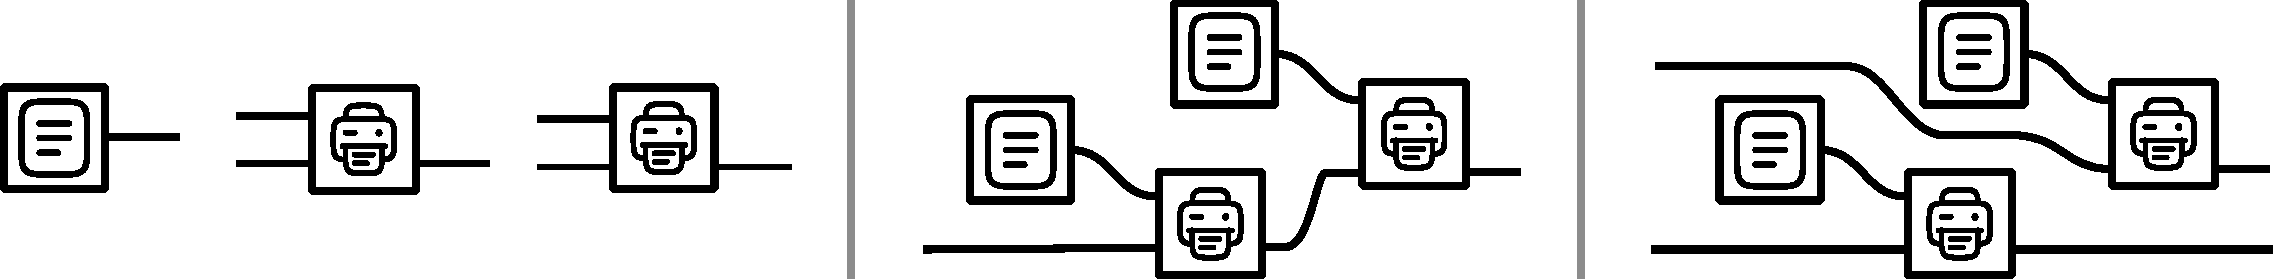
\includegraphics[width=0.95\linewidth,height=0.4\textheight,keepaspectratio]{graphic-01.pdf}\end{center}
 
Figure 1: (Left) An effectful signature. (Center) Resourceful trace over the first two elements of the effectful signature, i.e. involving only one printer. (Right) Resourceful trace involving two printers: printings are now independent of one another.\par
 
% END S1.F1
 
% BEGIN S1.p6
 
If we only admit one printer in our system, printing actions must occur in a specific order, and this is captured by the topology of the trace, as in the center of Figure 1. However, if we admit both printers, printing can occur concurrently, and this is again captured by the topology of the traces, such as on the right of Figure 1, where the printing actions may slide past one another or interchange. We shall see in Section 5 that this example in fact arises by a canonical combination of the “theory of a printer” with itself, called the commuting tensor product, generalizing the commuting tensor product of algebraic theories [9].\par
 
% END S1.p6
 
% BEGIN S1.p7
 
The collection of all resourceful traces over an effectful signature assembles into an effectful category [23], also known as generalized Freyd categories [10, 21], a well-known algebraic structure in the semantics of effectful computation. Indeed, one of the results of this paper is that resourceful traces are the morphisms in free effectful categories. That is, we show that there is an adjunction between effectful signatures and effectful categories, generalizing the classic maximal cliques construction for Mazurkiewicz traces.\par
 
% END S1.p7
 
% BEGIN S1.SS0.SSS0.Px1
 
\par\medskip\noindent\textbf{Related work}\par
 
% BEGIN S1.SS0.SSS0.Px1.p1
 
That Mazurkiewicz traces can be seen as morphisms in certain free monoidal categories was elaborated by Sobociński and the first author [7]. By moving to effectful categories, we sharpen this viewpoint, recovering Mazurkiewicz traces precisely as the morphisms in free effectful categories with no resources (qua “indefinite noun phrases”). The construction of free effectful categories over effectful signatures with a single device was given by the third author, following Jeffrey [13, 22, 23]. The construction of the commuting tensor product of effectful categories appeared in [6], in terms of string diagrams, covering the case of morphisms supported by a finite number of devices. The central results of this paper are new, namely the existence of an adjunction between effectful signatures and effectful categories (Corollary 42), and Theorem 47 on the commuting tensor product of free effectful categories.\par
 
% END S1.SS0.SSS0.Px1.p1
 
% END S1.SS0.SSS0.Px1
 
% BEGIN S1.SS0.SSS0.Px2
 
\par\medskip\noindent\textbf{Outline}\par
 
% BEGIN S1.SS0.SSS0.Px2.p1
 
Section 2 recalls the notion of Mazurkiewicz trace, and their graphical representation. Section 3 introduces effectful signatures and effectful categories, via their underlying device signatures and monoidal signatures, generalizing the notion of distribution of an alphabet of actions. We give a construction of the free effectful category over an effectful signature, whose morphisms are resourceful traces. In Section 4, we show how the cliques construction from the theory of traces generalizes to effectful categories, and exhibits the free construction as a left adjoint. Finally, Section 5 gives a construction of the commuting tensor product of free effectful categories, capturing the combination of systems in which the morphisms of each are forced to commute with one another, even while they may exchange resources.\par
 
% END S1.SS0.SSS0.Px2.p1
 
% END S1.SS0.SSS0.Px2
 
% END S1


% BEGIN S2
 
\par\medskip\noindent\textbf{2 Mazurkiewicz traces}\par
 
% BEGIN S2.p1
 
In this section, we recall the basic definitions of trace theory, including the graphical presentation of traces. For more details, we refer to Mazurkiewicz, Hoogeboom and Rozenberg [5]. For this section, we fix a set of actions $\Sigma$, and denote by $\Sigma^{*}$ the monoid of words over $\Sigma$.\par
 
% END S2.p1
 
% BEGIN Thmtheorem1
 
\par\medskip\noindent\textbf{Definition 1.}\par
 
% BEGIN Thmtheorem1.p1
 
A dependency relation, $D\subseteq\Sigma\times\Sigma$, is a reflexive, symmetric relation. Dependency relations form a preorder, $\mathsf{Dep}_{\Sigma}$, with order the inclusion of relations.\par
 
% END Thmtheorem1.p1
 
% END Thmtheorem1
 
% BEGIN S2.p2
 
Intuitively, a dependency relation specifies actions which should not occur concurrently, because they have some kind of dependency on each other, or the potential to interfere, such as writing to the same location in memory.\par
 
% END S2.p2
 
% BEGIN Thmtheorem2
 
\par\medskip\noindent\textbf{Definition 2.}\par
 
% BEGIN Thmtheorem2.p1
 
Given a dependency relation $D\subseteq\Sigma\times\Sigma$, let $\equiv_{D}$ be the least congruence on $\Sigma^{*}$ such that for every pair of actions $a,b\in D$, $(a,b)\notin D$ implies $ab\equiv_{D}ba$. The free partially commutative monoid or trace monoid generated by $D$ is the quotient monoid $\Sigma^{*}/{\equiv_{D}}$. An element of the trace monoid is a Mazurkiewicz trace (or simply trace) over $(\Sigma,D)$.\par
 
% END Thmtheorem2.p1
 
% END Thmtheorem2
 
% BEGIN S2.p3
 
A trace is thus an equivalence class of words up to commutation of independent actions. Another construction of traces starts from distributions of the set of actions:\par
 
% END S2.p3
 
% BEGIN Thmtheorem3
 
\par\medskip\noindent\textbf{Definition 3.}\par
 
% BEGIN Thmtheorem3.p1
 
A distribution of $\Sigma$ is a function $\mathsf{dev}:\Sigma\to\mathscr{P}(\{1,...,k\})$ for some $k\geqslant 1$. Distributions form a preorder $\mathsf{Dist}_{\Sigma}$ with $\mathsf{dev}\leqslant\mathsf{dev}^{\prime}$ if and only if for all $a,b\in\Sigma$, $\mathsf{dev}(a)\cap\mathsf{dev}(b)=\varnothing\implies\mathsf{dev}^{\prime}(a)\cap\mathsf{dev}^{\prime}(b)=\varnothing.$\par
 
% END Thmtheorem3.p1
 
% END Thmtheorem3
 
% BEGIN S2.p4
 
Classically, $\mathsf{dev}(\sigma)$ is known as the set of locations of $\sigma$. In line with the terminology introduced in the following, we call $\mathsf{dev}(\sigma)$ the set of devices of $\sigma$. In terms of concurrency, we might consider $\mathsf{dev}(\sigma)$ to be the set of shared resources on which $\sigma$ depends, such as memory locations, execution threads, runtimes or peripherals.\par
 
% END S2.p4
 
% BEGIN S2.p5
 
We can represent a distribution graphically by introducing nodes (depicted as boxes) corresponding to actions in $\Sigma$, with interfaces (depicted as patterned strings) corresponding to the devices assigned to the action, as for example in Figure 2.\par
 
% END S2.p5
 
% BEGIN S2.F2

\begin{center}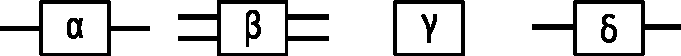
\includegraphics[width=0.95\linewidth,height=0.4\textheight,keepaspectratio]{graphic-02.pdf}\end{center}
 
Figure 2: Graphical representation of a distribution: $\alpha$ and $\beta$ share one device, and $\beta$ and $\delta$ share one device, whereas $\gamma$ has no devices.\par
 
% END S2.F2
 
% BEGIN S2.p6
 
Traces are the diagrams that we can build by plugging these components together, subject to the restriction that each device string occurs exactly once in each vertical slice of the diagram, such as in Figure 3. This is formalized by the algebra of (pre)monoidal categories, as we shall see in the next section. The collection of all such diagrams also forms a monoid, isomorphic to the trace monoid. More details can be found in the work of Sobociński and the first author [7], which builds on earlier work on the representation of traces as graphs [5].\par
 
% END S2.p6
 
% BEGIN S2.F3

\begin{center}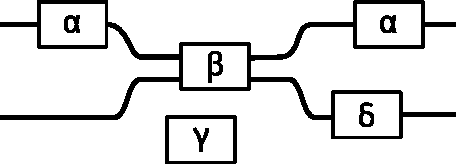
\includegraphics[width=0.95\linewidth,height=0.4\textheight,keepaspectratio]{graphic-03.pdf}\end{center}
 
Figure 3: Graphical representation of a trace over the distribution in Figure 2. As an equivalence class of words in the trace monoid, this trace would include for example $\gamma\alpha\beta\alpha\delta$ and $\alpha\beta\gamma\delta\alpha$: independence is captured by sliding actions, while keeping the boundaries fixed.\par
 
% END S2.F3
 
% BEGIN S2.p7
 
A classical construction lets us move between dependency relations and distributions: devices correspond to (non-trivial) maximal cliques in the graph of the dependency relation. For example, the dependency relation depicted in Figure 4 gives rise to the distribution in Figure 2. In Section 4, we shall apply a similar construction to effectful categories.\par
 
% END S2.p7
 
% BEGIN Thmtheorem4
 
\par\medskip\noindent\textbf{Definition 4.}\par
 
% BEGIN Thmtheorem4.p1
 
The graph of a dependency relation $\Sigma\subseteq D\times D$ has vertices the elements of $\Sigma$ and an edge $(a,b)$ for every $(a,b)\in D$.\par
 
% END Thmtheorem4.p1
 
% END Thmtheorem4
 
% BEGIN S2.F4

\begin{center}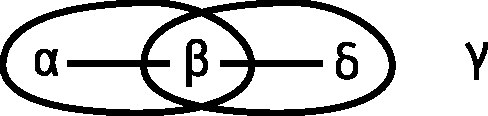
\includegraphics[width=0.95\linewidth,height=0.4\textheight,keepaspectratio]{graphic-04.pdf}\end{center}
 
Figure 4: Graph of a dependency relation, whose indicated non-trivial maximal cliques give rise to the distribution of Figure 2.\par
 
% END S2.F4
 
% BEGIN Thmtheorem5
 
\par\medskip\noindent\textbf{Proposition 5.}\par
 
% BEGIN Thmtheorem5.p1
 
([7, §4.1]) Every dependency relation $D$ on $\Sigma$ gives rise to a distribution of $\Sigma$ by taking a bijection of $\{1,...,k\}$ with the non-trivial maximal cliques of the graph of $D$, with $\mathsf{dev}$ sending an action to the subset of such cliques to which it belongs. This extends to a (contravariant) Galois insertion, $\mathsf{cliques}\colon\mathsf{Dep}_{\Sigma}\hookrightarrow\mathsf{Dist}_{\Sigma}$.\par
 
% END Thmtheorem5.p1
 
% END Thmtheorem5
 
% BEGIN S2.p8
 
Finally, we remark that any monoid has an underlying distribution, which can be found using the maximal cliques construction. A monoid $M$ has a dependency relation $D$ on its elements defined by $(a,b)\in D$ just when $a$ and $b$ do not commute in $M$, and taking non-trivial maximal cliques in the graph of this dependency relation defines a distribution of $M$. We shall extend this idea to effectful categories in Section 4.\par
 
% END S2.p8
 
% END S2


% BEGIN S3
 
\par\medskip\noindent\textbf{3 Resourceful traces and free effectful categories}\par
 
% BEGIN S3.p1
 
In traces, actions are merely atomic names, equipped with a set of devices. In this section, we enrich the language of traces by allowing actions to additionally have input and output types, which we think of as resources that may be shared between actions. Actions therefore become morphisms, with a designated source and target.\par
 
% END S3.p1
 
% BEGIN S3.p2
 
In Section 3.1, we introduce the resourceful analogue of the distribution of a set of actions, which we call an effectful signature. In an effectful signature, in addition to a set of devices, every action is equipped with input and output types of resources. In Section 3.3, we show that just as a distribution generates a free partially commutative monoid, effectful signatures generate free effectful categories [23], also known as generalized Freyd categories [10, 21].\par
 
% END S3.p2
 
% BEGIN S3.SS1
 
\par\medskip\noindent\textbf{3.1 Effectful signatures}\par
 
% BEGIN S3.SS1.p1
 
Effectful signatures refine distributions: not only by equipping actions with input and output types, but additionally by designating some central or pure actions, with only the impure actions being potentially able to interfere. In programming language theory, this is the division between values and computations [19, 15].\par
 
% END S3.SS1.p1
 
% BEGIN S3.SS1.p2
 
One reason for this can be seen already at the level of trace monoids. Morphisms of trace monoids are, a priori, simply morphisms of monoids, but these need not preserve centrality of actions. That is, if an action $\alpha$ commutes with all actions in a trace monoid $M$ (i.e., $\alpha$ is central in $M$), then its image under a monoid homomorphism $M\to N$ need not commute with all actions of $N$. Thus, certain actions that we might consider to be pure might change their role under a translation of systems. However, restricting the notion of morphism to require preservation of centrality is too strong, since it is possible for computations to be incidentally central: an example may be found in Staton and Levy [24, §5.2].\par
 
% END S3.SS1.p2
 
% BEGIN S3.SS1.p3
 
To overcome this, we explicitly designate which actions we want to consider as pure, and ask that centrality of just these actions is preserved. The chosen set of pure actions is specified by a monoidal signature:\par
 
% END S3.SS1.p3
 
% BEGIN Thmtheorem6
 
\par\medskip\noindent\textbf{Definition 6.}\par
 
% BEGIN Thmtheorem6.p1
 
A monoidal signature $M$ consists of a set of objects, $V_{M}$; a set of arrows, $E_{M}$; and a pair of functions $\delta_{0},\delta_{1}:E_{M}\to V_{M}^{*}$ assigning source and target lists of objects to each arrow. We can equivalently present a monoidal signature by a set of objects $V_{M}$, and sets $M(X_{1},...,X_{n};Y_{1},...,Y_{m})$ of arrows for each pair of lists of objects: we shall find both perspectives useful.\par
 
% END Thmtheorem6.p1
 
% END Thmtheorem6
 
% BEGIN S3.SS1.p4
 
We can picture a monoidal signature as on the left of Figure 5, where boxes depict the arrows, and their associated strings designate the sources and targets. We use solid strings for the objects of a monoidal signature.\par
 
% END S3.SS1.p4
 
% BEGIN Thmtheorem7
 
\par\medskip\noindent\textbf{Definition 7.}\par
 
% BEGIN Thmtheorem7.p1
 
A morphism of monoidal signatures $\alpha:M\to N$ comprises two functions $\alpha_{E}:E_{M}\to E_{N}$ and $\alpha_{V}:V_{M}\to V_{N}$ commuting with $\delta_{0}$ and $\delta_{1}$, that is, $\delta_{i}\mathop{\fatsemi}\alpha_{V}^{*}=\alpha_{E}\mathop{\fatsemi}\delta_{i}$.\par
 
% END Thmtheorem7.p1
 
% BEGIN Thmtheorem7.p2
 
Equivalently, a morphism is specified by a function $\alpha$ on objects, and functions\par
    \[M(X_{1},...,X_{n};Y_{1},...,Y_{m})\to N(\alpha X_{1},...,\alpha X_{n};\alpha Y_{1},...,\alpha Y_{m}).\]    
% END Thmtheorem7.p2
 
% BEGIN Thmtheorem7.p3
 
It is easy to check that morphisms of monoidal signatures compose, the composite given by composing their underlying actions on arrows and objects, and that we have identities. Denote by $\mathsf{MonGraph}$ the category of monoidal signatures and their morphisms.\par
 
% END Thmtheorem7.p3
 
% END Thmtheorem7
 
% BEGIN S3.SS1.p5
 
The set of morphisms that may be equipped with devices, specifying dependencies between morphisms, is given by a device signature, which is simply a monoidal signature together with extra data associating a set of devices to each morphism:\par
 
% END S3.SS1.p5
 
% BEGIN Thmtheorem8
 
\par\medskip\noindent\textbf{Definition 8.}\par
 
% BEGIN Thmtheorem8.p1
 
A device signature $C$ comprises\par
  
\par\noindent  $\blacksquare$ 
% BEGIN S3.I1.i1.p1
 
a monoidal signature $|C|$,\par
 
% END S3.I1.i1.p1
 
 
\par\noindent  $\blacksquare$ 
% BEGIN S3.I1.i2.p1
 
a set $\mathcal{D}_{C}$ of devices, and\par
 
% END S3.I1.i2.p1
 
 
\par\noindent  $\blacksquare$ 
% BEGIN S3.I1.i3.p1
 
a function $\mathsf{dev}_{C}:E_{|C|}\to\mathcal{P}(\mathcal{D}_{C})$ assigning each arrow in $|C|$ to a subset of the devices. We shall simply write $\mathsf{dev}$ when the device signature $C$ is clear from context.\par
 
% END S3.I1.i3.p1
 
  
% END Thmtheorem8.p1
 
% END Thmtheorem8
  
% BEGIN S3.F5

\begin{center}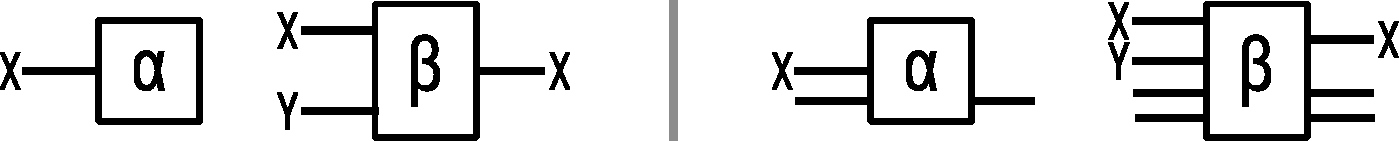
\includegraphics[width=0.95\linewidth,height=0.4\textheight,keepaspectratio]{graphic-05.pdf}\end{center}
 
Figure 5: Left: monoidal signature with arrows $\alpha:X\to\varepsilon$, $\beta:XY\to X$. Right: device signature with the same underlying monoidal signature as on the left. $\alpha$ and $\beta$ share a device, but $\beta$ has an additional device. The devices of an action all appear in both the source and target, but need not occur in a specific order.\par
 
% END S3.F5
 
% BEGIN S3.SS1.p6
 
When a generator has a finite subset of devices, we can depict a device signature as on the right of Figure 5. Patterned strings denote devices (with arbitrary order of appearance). In contrast to resource strings, device strings must thread through the process: this enforces a definite ordering of dependent processes.\par
 
% END S3.SS1.p6
 
% BEGIN Thmtheorem9
 
\par\medskip\noindent\textbf{Example 9.}\par
 
% BEGIN Thmtheorem9.p1
 
A device signature in which the underlying monoidal signature has an empty set of objects and set of arrows $\Sigma$ is precisely a distribution of $\Sigma$ in the sense of Definition 3, although we allow the set of devices to be infinite. In practice, a finite set of devices often suffices. For example, if the device signature has a finite number of arrows, then an infinite number of devices can be shown to be redundant.\par
 
% END Thmtheorem9.p1
 
% END Thmtheorem9
 
% BEGIN Thmtheorem10
 
\par\medskip\noindent\textbf{Definition 10.}\par
 
% BEGIN Thmtheorem10.p1
 
Morphisms $f$ and $g$ in a device signature $C$ are said to be orthogonal, denoted $f\perp_{C}g$ just when they share no devices, $\mathsf{dev}(f)\cap\mathsf{dev}(g)=\varnothing$. Note that any $f$ with no devices is orthogonal to every $g$. We write $f\perp g$ when $C$ is clear from context, and $f\mathbin{\rotatebox{90.0}{$\nvdash$}}g$ when $f$ and $g$ are not orthogonal.\par
 
% END Thmtheorem10.p1
 
% END Thmtheorem10
 
% BEGIN S3.SS1.p7
 
A morphism of device signatures must preserve orthogonality, that is\par
 
% END S3.SS1.p7
 
% BEGIN Thmtheorem11
 
\par\medskip\noindent\textbf{Definition 11.}\par
 
% BEGIN Thmtheorem11.p1
 
A morphism of device signatures, $\alpha:C\to D$, comprises\par
  
\par\noindent  $\blacksquare$ 
% BEGIN S3.I2.i1.p1
 
a morphism of underlying monoidal signatures, $\alpha:|C|\to|D|$,\par
 
% END S3.I2.i1.p1
 
 
\par\noindent  $\blacksquare$ 
% BEGIN S3.I2.i2.p1
 
such that for all arrows $f,g\in C$, if $f\mathbin{{\color[rgb]{0.296875,0.3359375,0.4140625}\definecolor[named]{pgfstrokecolor}{rgb}{0.296875,0.3359375,0.4140625}\perp}_{C}}g$ then $\alpha(f)\mathbin{{\color[rgb]{0.296875,0.3359375,0.4140625}\definecolor[named]{pgfstrokecolor}{rgb}{0.296875,0.3359375,0.4140625}\perp}_{D}}\alpha(g)$.\par
 
% END S3.I2.i2.p1
 
  
% END Thmtheorem11.p1
 
% END Thmtheorem11
 
% BEGIN S3.SS1.p8
 
Composition of these morphisms is given by composition of their underlying morphisms of monoidal signatures. It is easily checked that preservation of orthogonality is satisfied by a composite, and so device signatures and their morphisms form a category $\mathsf{DevGraph}$.\par
 
% END S3.SS1.p8
 
% BEGIN S3.SS1.p9
 
We now have the ingredients required to define effectful signatures.\par
 
% END S3.SS1.p9
 
% BEGIN Thmtheorem12
 
\par\medskip\noindent\textbf{Definition 12.}\par
 
% BEGIN Thmtheorem12.p1
 
An effectful signature $\mathcal{G}:V\to C$ comprises\par
  
\par\noindent  $\blacksquare$ 
% BEGIN S3.I3.i1.p1
 
a monoidal signature $V$,\par
 
% END S3.I3.i1.p1
 
 
\par\noindent  $\blacksquare$ 
% BEGIN S3.I3.i2.p1
 
a device signature $C$ over the same set of objects as $V$,\par
 
% END S3.I3.i2.p1
 
 
\par\noindent  $\blacksquare$ 
% BEGIN S3.I3.i3.p1
 
an identity-on-objects morphism of monoidal signatures $\mathcal{G}:V\to|C|$,\par
 
% END S3.I3.i3.p1
 
 
\par\noindent  $\blacksquare$ 
% BEGIN S3.I3.i4.p1
 
such that $\mathsf{dev}(\mathcal{G}v)=\varnothing$ for all arrows $v$ in $V$.\par
 
% END S3.I3.i4.p1
 
  
% END Thmtheorem12.p1
 
% END Thmtheorem12
 
% BEGIN S3.SS1.p10
 
We usually think of $V$ in terms of its image in $C$, and thus when we speak of a morphism in an effectful signature, we are referring to the arrows of the device signature $C$.\par
 
% END S3.SS1.p10
 
% BEGIN Thmtheorem13
 
\par\medskip\noindent\textbf{Example 13.}\par
 
% BEGIN Thmtheorem13.p1
 
In the effectful signature in Figure 1, the monoidal signature comprises solely the “document” generator, while the device signature includes all three generators, with the morphism of monoidal signatures simply including the “document” generator.\par
 
% END Thmtheorem13.p1
 
% END Thmtheorem13
 
% BEGIN Thmtheorem14
 
\par\medskip\noindent\textbf{Definition 14.}\par
 
% BEGIN Thmtheorem14.p1
 
A morphism of effectful signatures $(\alpha_{0},\alpha):(\mathcal{G}:V\to C)\to(\mathcal{H}:W\to D)$ comprises\par
  
\par\noindent  $\blacksquare$ 
% BEGIN S3.I4.i1.p1
 
a morphism of monoidal signatures $\alpha_{0}:V\to W$, and\par
 
% END S3.I4.i1.p1
 
 
\par\noindent  $\blacksquare$ 
% BEGIN S3.I4.i2.p1
 
a morphism of device signatures $\alpha:C\to D$,\par
 
% END S3.I4.i2.p1
 
 
\par\noindent  $\blacksquare$ 
% BEGIN S3.I4.i3.p1
 
such that the square of morphisms of monoidal signatures commutes, $\mathcal{G}\mathop{\fatsemi}\alpha=\alpha_{0}\mathop{\fatsemi}\mathcal{H}$.\par
 
% END S3.I4.i3.p1
 
  
% END Thmtheorem14.p1
 
% END Thmtheorem14
 
% BEGIN S3.SS1.p11
 
Since both $\mathsf{MonGraph}$ and $\mathsf{DevGraph}$ are categories, it follows easily that\par
 
% END S3.SS1.p11
 
% BEGIN Thmtheorem15
 
\par\medskip\noindent\textbf{Proposition 15.}\par
 
% BEGIN Thmtheorem15.p1
 
Effectful signatures and their morphisms form a category $\mathsf{EffGraph}$.\par
 
% END Thmtheorem15.p1
 
% END Thmtheorem15
 
% BEGIN S3.SS1.p12
 
Note that effectful signatures generalize the effectful polygraphs of Sobociński and the third author [23], precisely by allowing each action to have a different set of devices, rather than all actions having a single, global device. The construction of effectful categories in the next section also refines that from effectful polygraphs [23], in that it builds in extra independence equations between processes.\par
 
% END S3.SS1.p12
 
% END S3.SS1
 
% BEGIN S3.SS2
 
\par\medskip\noindent\textbf{3.2 Effectful categories}\par
 
% BEGIN S3.SS2.p1
 
Effectful signatures generate effectful categories. An effectful category comprises a monoidal category $\mathbb{V}$, a premonoidal category $\mathbb{C}$, and an identity-on-objects premonoidal functor $\mathbb{V}\to\mathbb{C}$. In this paper, we work with strict versions of these notions, since not only are the free such structures strict, but coherence theorems exist which state that any (pre)monoidal category is equivalent to a strict one [20].\par
 
% END S3.SS2.p1
 
% BEGIN S3.SS2.p2
 
Just as with effectful signatures, the idea is that $\mathbb{V}$ is a category of pure actions (generated by a monoidal signature), $\mathbb{C}$ is a category of effectful actions (generated by a device signature), and the functor is thought of as an inclusion of $\mathbb{V}$ into $\mathbb{C}$. Let us build up to their definition.\par
 
% END S3.SS2.p2
 
% BEGIN Thmtheorem16
 
\par\medskip\noindent\textbf{Definition 16.}\par
 
% BEGIN Thmtheorem16.p1
 
A strict monoidal category is a category $\mathbb{V}$ equipped with\par
  
\par\noindent  $\blacksquare$ 
% BEGIN S3.I5.i1.p1
 
a functor $\otimes:\mathbb{V}\times\mathbb{V}\to\mathbb{V}$, called the monoidal product,\par
 
% END S3.I5.i1.p1
 
 
\par\noindent  $\blacksquare$ 
% BEGIN S3.I5.i2.p1
 
a distinguished object $I$, called the monoidal unit,\par
 
% END S3.I5.i2.p1
 
 
\par\noindent  $\blacksquare$ 
% BEGIN S3.I5.i3.p1
 
such that $A\otimes(B\otimes C)=(A\otimes B)\otimes C$ and $A\otimes I=A=I\otimes A$,\par
 
% END S3.I5.i3.p1
 
 
\par\noindent  $\blacksquare$ 
% BEGIN S3.I5.i4.p1
 
and such that the following equations hold for all morphisms $f,g,h$:\par
    \[f\otimes(g\otimes h)=(f\otimes g)\otimes h\\
1_{I}\otimes f=f=f\otimes 1_{I}.\]    
% END S3.I5.i4.p1
 
  
% END Thmtheorem16.p1
 
% END Thmtheorem16
 
% BEGIN S3.SS2.p3
 
Premonoidal categories refine monoidal categories by only requiring the monoidal product to be functorial separately in each variable: in particular, there is no operation combining arbitrary morphisms in parallel.\par
 
% END S3.SS2.p3
 
% BEGIN Thmtheorem17
 
\par\medskip\noindent\textbf{Definition 17.}\par
 
% BEGIN Thmtheorem17.p1
 
A strict premonoidal category is a category, $\mathbb{C}$, equipped with functors $(A\ltimes-):\mathbb{C}\to\mathbb{C}$ (the “left-whiskering” by A) and $(-\rtimes A):\mathbb{C}\to\mathbb{C}$ (the “right-whiskering” by A), for every object $A$ of $\mathbb{C}$, and a distinguished object $I$ (the “monoidal unit”), such that,\par
  
\par\noindent  $\blacksquare$ 
% BEGIN S3.I6.i1.p1
 
$A\rtimes B=A\ltimes B$, allowing us to denote this object as $A\otimes B$,\par
 
% END S3.I6.i1.p1
 
 
\par\noindent  $\blacksquare$ 
% BEGIN S3.I6.i2.p1
 
$A\otimes(B\otimes C)=(A\otimes B)\otimes C$ and $A\otimes I=A=I\otimes A$,\par
 
% END S3.I6.i2.p1
 
 
\par\noindent  $\blacksquare$ 
% BEGIN S3.I6.i3.p1
 
and such that the following equations hold, stating coherence of left- and right-whiskering with each other and with the monoid structure\par
    $\displaystyle(A\ltimes f)\rtimes B=A\ltimes(f\rtimes B)\qquad I\ltimes f=f=f\rtimes
I$     $\displaystyle(A\otimes B)\ltimes f=A\ltimes(B\ltimes f)\qquad f\rtimes(A\otimes B)=(f\rtimes A)\rtimes B.$    
% END S3.I6.i3.p1
 
% BEGIN S3.I6.i3.p2
 
\par
 
% END S3.I6.i3.p2
 
  
% END Thmtheorem17.p1
 
% END Thmtheorem17
 
% BEGIN S3.SS2.p4
 
Note that every monoidal category is a premonoidal category in which partial applications of the monoidal product define the left- and right- whiskerings. The key equations that hold for every pair of morphisms in a monoidal category, but not generally in a given premonoidal category, are those expressing interchange (i.e., commutation) of morphisms:\par
 
% END S3.SS2.p4
 
% BEGIN Thmtheorem18
 
\par\medskip\noindent\textbf{Definition 18.}\par
 
% BEGIN Thmtheorem18.p1
 
For morphisms $f:A\to B$ and $g:A^{\prime}\to B^{\prime}$ in a premonoidal category $\mathbb{C}$,\par
  
\par\noindent  $\blacksquare$ 
% BEGIN S3.I7.i1.p1
 
we write $f{\color[rgb]{0,0,1}\definecolor[named]{pgfstrokecolor}{rgb}{0,0,1}\parallel}g$ in case $(f\rtimes A^{\prime})(B\ltimes g)=(A\ltimes g)(f\rtimes B^{\prime})$,\par
 
% END S3.I7.i1.p1
 
 
\par\noindent  $\blacksquare$ 
% BEGIN S3.I7.i2.p1
 
we say that $f$ and $g$ interchange in case $f\parallel g$ and $g\parallel f$,\par
 
% END S3.I7.i2.p1
 
 
\par\noindent  $\blacksquare$ 
% BEGIN S3.I7.i3.p1
 
we say that $f$ and $g$ interfere, written $f\lightning g$, in case they do not interchange,\par
 
% END S3.I7.i3.p1
 
 
\par\noindent  $\blacksquare$ 
% BEGIN S3.I7.i4.p1
 
we say that $f$ is central in case it interchanges with every morphism of $\mathbb{C}$.\par
 
% END S3.I7.i4.p1
 
  
% END Thmtheorem18.p1
 
% END Thmtheorem18
 
% BEGIN S3.SS2.p5
 
Graphically, interchange of morphisms is precisely the sliding of morphisms past one another, as discussed for example in Figure 3.\par
 
% END S3.SS2.p5
 
% BEGIN Thmtheorem19
 
\par\medskip\noindent\textbf{Definition 19.}\par
 
% BEGIN Thmtheorem19.p1
 
Let $\mathbb{C}$ and $\mathbb{D}$ be strict premonoidal categories. A strict premonoidal functor is a functor $F:\mathbb{C}\to\mathbb{D}$ that\par
  
\par\noindent  $\blacksquare$ 
% BEGIN S3.I8.i1.p1
 
maps objects as a monoid homomorphism, $F(A\otimes B)=F(A)\otimes F(B)$ and $F(I)=I$,\par
 
% END S3.I8.i1.p1
 
 
\par\noindent  $\blacksquare$ 
% BEGIN S3.I8.i2.p1
 
and preserves whiskerings, $F(A\ltimes f)=F(A)\ltimes F(f)$ and $F(f\rtimes A)=F(f)\rtimes F(A)$.\par
 
% END S3.I8.i2.p1
 
  
When $\mathbb{C}$ and $\mathbb{D}$ are moreover strict monoidal categories, we call this a strict monoidal functor.\par
 
% END Thmtheorem19.p1
 
% END Thmtheorem19
 
% BEGIN S3.SS2.p6
 
Strict monoidal categories and strict premonoidal categories, along with strict functors form categories, ${\color[rgb]{0,0,1}\definecolor[named]{pgfstrokecolor}{rgb}{0,0,1}\mathsf{MonCat}}$ and ${\color[rgb]{0,0,1}\definecolor[named]{pgfstrokecolor}{rgb}{0,0,1}\mathsf{PremonCat}}$. Finally, we reach the definition of effectful categories:\par
 
% END S3.SS2.p6
 
% BEGIN Thmtheorem20
 
\par\medskip\noindent\textbf{Definition 20.}\par
 
% BEGIN Thmtheorem20.p1
 
A (strict) effectful category $\mathscr{E}:\mathbb{V}\to\mathbb{C}$ comprises\par
  
\par\noindent  $\blacksquare$ 
% BEGIN S3.I9.i1.p1
 
a strict monoidal category $\mathbb{V}$,\par
 
% END S3.I9.i1.p1
 
 
\par\noindent  $\blacksquare$ 
% BEGIN S3.I9.i2.p1
 
a strict premonoidal category $\mathbb{C}$ with the same objects as $\mathbb{V}$, $\mathbb{C}_{\mathsf{obj}}=\mathbb{V}_{\mathsf{obj}}$,\par
 
% END S3.I9.i2.p1
 
 
\par\noindent  $\blacksquare$ 
% BEGIN S3.I9.i3.p1
 
an identity-on-objects strict premonoidal functor $\mathscr{E}:\mathbb{V}\to\mathbb{C}$,\par
 
% END S3.I9.i3.p1
 
 
\par\noindent  $\blacksquare$ 
% BEGIN S3.I9.i4.p1
 
such that the image of $\mathscr{E}:\mathbb{V}\to\mathbb{C}$ is central.\par
 
% END S3.I9.i4.p1
 
  
% END Thmtheorem20.p1
 
% END Thmtheorem20
 
% BEGIN Thmtheorem21
 
\par\medskip\noindent\textbf{Definition 21.}\par
 
% BEGIN Thmtheorem21.p1
 
A morphism of (strict) effectful categories, $(\alpha_{0},\alpha):(\mathscr{E}:\mathbb{V}\to\mathbb{C})\to(\mathscr{F}:\mathbb{W}\to\mathbb{D})$, comprises a strict monoidal functor $\alpha_{0}:\mathbb{V}\to\mathbb{W}$ and a strict premonoidal functor $\alpha:\mathbb{C}\to\mathbb{D}$ such that $\mathscr{E}\mathop{\fatsemi}\alpha=\alpha_{0}\mathop{\fatsemi}\mathscr{F}$ in ${\color[rgb]{0.296875,0.3359375,0.4140625}\definecolor[named]{pgfstrokecolor}{rgb}{0.296875,0.3359375,0.4140625}\mathsf{PremonCat}}$ (eliding the inclusion of ${\color[rgb]{0.296875,0.3359375,0.4140625}\definecolor[named]{pgfstrokecolor}{rgb}{0.296875,0.3359375,0.4140625}\mathsf{MonCat}}\hookrightarrow{\color[rgb]{0.296875,0.3359375,0.4140625}\definecolor[named]{pgfstrokecolor}{rgb}{0.296875,0.3359375,0.4140625}\mathsf{PremonCat}}$).\par
 
% END Thmtheorem21.p1
 
% END Thmtheorem21
 
% BEGIN S3.SS2.p7
 
From the fact that ${\color[rgb]{0.296875,0.3359375,0.4140625}\definecolor[named]{pgfstrokecolor}{rgb}{0.296875,0.3359375,0.4140625}\mathsf{MonCat}}$ and ${\color[rgb]{0.296875,0.3359375,0.4140625}\definecolor[named]{pgfstrokecolor}{rgb}{0.296875,0.3359375,0.4140625}\mathsf{PremonCat}}$ are categories, it follows easily that:\par
 
% END S3.SS2.p7
 
% BEGIN Thmtheorem22
 
\par\medskip\noindent\textbf{Proposition 22.}\par
 
% BEGIN Thmtheorem22.p1
 
Effectful categories and their morphisms form a category $\mathsf{EffCat}$.\par
 
% END Thmtheorem22.p1
 
% END Thmtheorem22
 
% END S3.SS2
 
% BEGIN S3.SS3
 
\par\medskip\noindent\textbf{3.3 Free effectful category over an effectful signature}\par
 
% BEGIN S3.SS3.p1
 
Our goal now is to define a functor $\mathscr{F}{}:\mathsf{EffGraph}\to\mathsf{EffCat}$. We will see in the next section that this functor has a right adjoint, and so constructs the free effectful category on an effectful signature. We begin with the free premonoidal category over a device signature.\par
 
% END S3.SS3.p1
 
% BEGIN Thmtheorem23
 
\par\medskip\noindent\textbf{Definition 23.}\par
 
% BEGIN Thmtheorem23.p1
 
For a device signature $G$, we construct a premonoidal category $\mathcal{F}G$ on $G$ as follows. The underlying category has,\par
  
\par\noindent  $\blacksquare$ 
% BEGIN S3.I10.i1.p1
 
set of objects $V_{G}^{*}$, the free monoid on $V_{G}$, whose elements are lists. We shall denote by $\otimes$ the concatenation of lists.\par
 
% END S3.I10.i1.p1
 
 
\par\noindent  $\blacksquare$ 
% BEGIN S3.I10.i2.p1
 
set of morphisms $E_{\mathcal{F}G}/{\equiv}$, where $E_{\mathcal{F}G}$ is the set inductively defined by rules for identities, the whiskering of generating arrows, and composition,\par
 
% END S3.I10.i2.p1
 
% BEGIN S3.I10.i2.p2
 
\begin{center}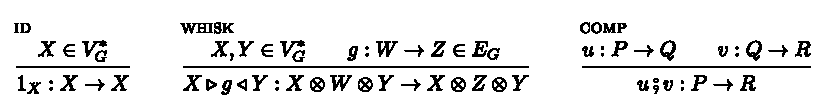
\includegraphics[width=0.95\linewidth,height=0.4\textheight,keepaspectratio]{graphic-06.pdf}\end{center}
 
% END S3.I10.i2.p2
 
 
\par\noindent  $\blacksquare$ 
% BEGIN S3.I10.i3.p1
 
and $\equiv$ is the least congruence for $\mathop{\fatsemi}$ generated by $(u\mathop{\fatsemi}v)\mathop{\fatsemi}w=u{\mathop{\fatsemi}}(v\mathop{\fatsemi}w),\,1_{X}\mathop{\fatsemi}u=u=u\mathop{\fatsemi}1_{Y}$\par
 
% END S3.I10.i3.p1
 
  
whenever these are well typed, along with equations allowing (whiskerings of) orthogonal generating arrows to interchange, i.e. for every pair, $f\colon U\to V$ and $g\colon U^{\prime}\to V^{\prime}$, of arrows in $E_{G}$ that are orthogonal, $\mathsf{dev}(f)\cap\mathsf{dev}(g)=\varnothing$, and each triple of objects $X,Y,Z$ in $V_{G}^{*}$,      $\displaystyle(X\triangleright f\triangleleft Y\otimes U^{\prime}\otimes Z)\mathop{\fatsemi}(X\otimes V\otimes Y\triangleright g\triangleleft Z)=(X\otimes U\otimes Y\triangleright g\triangleleft Z)\mathop{\fatsemi}(X\triangleright f\triangleleft Y\otimes V^{\prime}\otimes Z).$\par
 
% END Thmtheorem23.p1
 
% BEGIN Thmtheorem23.p2
 
It is immediate that this data forms a category. For the premonoidal structure, we define $I$ to be the empty list, left and right whiskerings act on objects by list concatenation (denoted $\otimes$), and their action on morphisms is defined inductively by\par
    \[(X\ltimes f):=\begin{cases}1_{X\otimes Y}&\text{if $f=1_{Y}$,}\\
(X\ltimes g){\mathop{\fatsemi}}(X\ltimes h)&\text{if $f=u{\mathop{\fatsemi}}v$,}\\
X\otimes Y\triangleright f^{\prime}\triangleleft Z&\text{if $f=Y\triangleright
f^{\prime}\triangleleft Z$,}\end{cases}\]       \[(f\rtimes X):=\begin{cases}1_{Y\otimes X}&\text{if $f=1_{Y}$,}\\
(g\rtimes X){\mathop{\fatsemi}}(h\rtimes X)&\text{if $f=u{\mathop{\fatsemi}}v$,}\\
Y\triangleright g\triangleleft Z\otimes X&\text{if $f=Y\triangleright g\triangleleft Z.$}\end{cases}\]    
% END Thmtheorem23.p2
 
% BEGIN Thmtheorem23.p3
 
It is easily verified that these mappings are well-defined, functorial, and satisfy the required coherence equations of Definition 17.\par
 
% END Thmtheorem23.p3
 
% END Thmtheorem23
 
% BEGIN S3.SS3.p2
 
The morphisms of $\mathcal{F}G$ are resourceful traces over $G$, and can be depicted intuitively as “string diagrams” (from an input boundary to an output boundary), built by combining whiskered generators of $G$ via the operations of premonoidal categories. Generators correspond to boxes as in Figure 5, identity morphisms correspond to strings, composition is given by joining resource strings and any matching device strings, leading to a morphism with the union of the two sets of devices, and whiskering by juxtaposing strings with boxes. Whiskering by the empty list is simply depicted by drawing no whiskering string. We illustrate this in Figure 6. The requirement that every device string appear at most once in every vertical slice through the diagram, as in Section 2, is enforced by the fact that we have no operation for combining morphisms in parallel. The following lemma shows that interchange of generating arrows extends to the morphisms of $\mathcal{F}G$ via the device assignment described above.\par
 
% END S3.SS3.p2
 
% BEGIN S3.F6

\begin{center}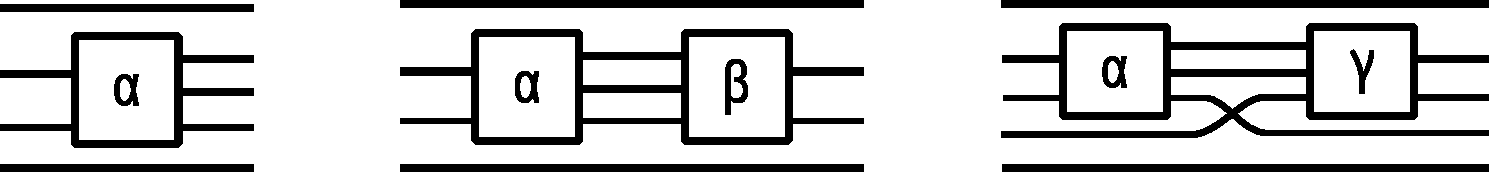
\includegraphics[width=0.95\linewidth,height=0.4\textheight,keepaspectratio]{graphic-07.pdf}\end{center}
 
Figure 6: (Left to right): Whiskering of a generating arrow by a resource, composition of morphisms with matching devices, composition of morphisms with distinct devices. Composition gives a morphism whose devices are the union of the components.\par
 
% END S3.F6
 
% BEGIN Thmtheorem24
 
\par\medskip\noindent\textbf{Definition 24.}\par
 
% BEGIN Thmtheorem24.p1
 
Device assignment extends inductively from a device signature $G$ to a well-defined function on the morphisms of $\mathcal{F}G$ (Definition 23) as follows\par
    \[\mathsf{dev}_{\mathcal{F}G}(f):=\begin{cases}\varnothing&\text{if $f=1_{A}$,}\\
\mathsf{dev}_{G}(f^{\prime})&\text{if $f=X\triangleright f^{\prime}\triangleleft Y$,}\\
\mathsf{dev}_{\mathcal{F}G}(g)\cup\mathsf{dev}_{\mathcal{F}G}(h)&\text{if $f=g{\mathop{\fatsemi}}h$.}\end{cases}\]    
% END Thmtheorem24.p1
 
% END Thmtheorem24
 
% BEGIN Thmtheorem25
 
\par\medskip\noindent\textbf{Lemma 25.}\par
 
% BEGIN Thmtheorem25.p1
 
Let $f,g$ be two morphisms of $\mathcal{F}G$. If $f$ and $g$ are orthogonal, $\mathsf{dev}_{\mathcal{F}G}(f)\cap\mathsf{dev}_{\mathcal{F}G}(g)=\varnothing$, then $f\parallel g$ and $g\parallel f$.\par
 
% END Thmtheorem25.p1
 
% END Thmtheorem25
 
% BEGIN S3.SS3.SSS0.P0.SPx1
 
\par\medskip\noindent\textbf{Proof.}\par
 
% BEGIN S3.SS3.SSS0.P0.SPx1.p1
 
See Appendix A. $\hfill\blacktriangleleft$\par
 
% END S3.SS3.SSS0.P0.SPx1.p1
 
% BEGIN Thmtheorem26
 
\par\medskip\noindent\textbf{Example 26.}\par
 
% BEGIN Thmtheorem26.p1
 
As noted in Example 9, a device signature $G$ with empty set of objects is precisely a distribution of an alphabet. In this case, $\mathcal{F}G$ has a single object, the empty list, and hence is a monoid (with trivial whiskerings). This monoid is isomorphic to the trace monoid over the corresponding distribution.\par
 
% END Thmtheorem26.p1
 
% END Thmtheorem26
 
% BEGIN Thmtheorem27
 
\par\medskip\noindent\textbf{Lemma 27.}\par
 
% BEGIN Thmtheorem27.p1
 
Each morphism of device signatures, $\alpha:G\to H$, induces a strict premonoidal functor, $\mathcal{F}(\alpha):\mathcal{F}G\to\mathcal{F}H$, defined as follows. The action on objects is the lifting of $\alpha_{V}$ to lists, $\alpha_{V}^{*}:V_{G}^{*}\to V_{H}^{*}$. The action on morphisms is given by\par
    \[\mathcal{F}(\alpha)(f):=\begin{cases}1_{\alpha^{*}(X)}&\text{if $f=1_{X}$},\\
\mathcal{F}(\alpha)(X)\triangleright\alpha_{E}(f^{\prime})\triangleleft\mathcal{F}(\alpha)(Y)&\text{if $f=X\triangleright f^{\prime}\triangleleft Y$}\\
\mathcal{F}(\alpha)(g)\mathop{\fatsemi}\mathcal{F}(\alpha)(h)&\text{if $f=g\mathop{\fatsemi}h$.}\\
\end{cases}\]    
and this action is well-defined.\par
 
% END Thmtheorem27.p1
 
% END Thmtheorem27
 
% END S3.SS3.SSS0.P0.SPx1
 
% BEGIN S3.SS3.SSS0.P0.SPx2
 
\par\medskip\noindent\textbf{Proof.}\par
 
% BEGIN S3.SS3.SSS0.P0.SPx2.p1
 
Well-definedness follows from the fact $\mathcal{F}G$ and $\mathcal{F}H$ are categories and that $\alpha$ preserves orthogonality by definition. The action on objects is a morphism of monoids, so to see that $\mathcal{F}(\alpha)$ is a strict premonoidal functor, it remains to check that it preserves whiskerings: this follows by a straightforward induction on $f$. $\hfill\blacktriangleleft$\par
 
% END S3.SS3.SSS0.P0.SPx2.p1
 
% BEGIN S3.SS3.SSS0.P0.SPx2.p2
 
It is clear that the mapping $\mathcal{F}$ preserves composition and identities, and thus\par
 
% END S3.SS3.SSS0.P0.SPx2.p2
 
% BEGIN Thmtheorem28
 
\par\medskip\noindent\textbf{Proposition 28.}\par
 
% BEGIN Thmtheorem28.p1
 
The assignments of Definition 23 and Lemma 27 define a functor $\mathcal{F}:\mathsf{DevGraph}\to\mathsf{PremonCat}$.\par
 
% END Thmtheorem28.p1
 
% END Thmtheorem28
 
% BEGIN S3.SS3.SSS0.P0.SPx2.p3
 
To define the free effectful category over an effectful signature, we simply combine the construction of the free monoidal category on a monoidal signature (Construction 48) with the construction of the free premonoidal category on a device signature (Definition 23), as follows.\par
 
% END S3.SS3.SSS0.P0.SPx2.p3
 
% BEGIN Thmtheorem29
 
\par\medskip\noindent\textbf{Definition 29.}\par
 
% BEGIN Thmtheorem29.p1
 
Let $\mathcal{G}:V\to C$ be an effectful signature. This generates the following effectful category $\mathscr{F}{\mathcal{G}}:\mathcal{F}_{\mathbin{\raisebox{1.25pt}{$\scriptscriptstyle\otimes$}}}V\to\mathcal{F}C$, which Proposition 30 checks is well-defined.\par
  
\par\noindent  $\blacksquare$ 
% BEGIN S3.I11.i1.p1
 
The monoidal category is the free monoidal category $\mathcal{F}_{\mathbin{\raisebox{1.25pt}{$\scriptscriptstyle\otimes$}}}V$ on the monoidal signature $V$,\par
 
% END S3.I11.i1.p1
 
 
\par\noindent  $\blacksquare$ 
% BEGIN S3.I11.i2.p1
 
the premonoidal category $\mathcal{F}{C}$ is the free premonoidal category on the device signature $C$,\par
 
% END S3.I11.i2.p1
 
 
\par\noindent  $\blacksquare$ 
% BEGIN S3.I11.i3.p1
 
$\mathscr{F}{\mathcal{G}}:\mathcal{F}_{\mathbin{\raisebox{1.25pt}{$\scriptscriptstyle\otimes$}}}V\to\mathcal{F}C$ is taken to be identity-on-objects, and is defined by structural induction on its arguments, following Construction 48. The interesting case is, for $g_{1}:A_{1}\to B_{1}$, $g_{2}:A_{2}\to B_{2}$,\par
    \[\mathscr{F}{\mathcal{G}}(g_{1}\otimes g_{2}):=(\mathscr{F}{\mathcal{G}}(g_{1})\rtimes A_{2})(B_{1}\ltimes\mathscr{F}{\mathcal{G}}(g_{2}))=(A_{1}\ltimes\mathscr{F}{\mathcal{G}}(g_{2}))(\mathscr{F}{\mathcal{G}}(g_{1})\rtimes B_{2}).\]    
For this equality to hold, we must have that $\mathscr{F}{\mathcal{G}}(g_{1})$ and $\mathscr{F}{\mathcal{G}}(g_{2})$ are orthogonal for all $g_{1}$ and $g_{2}$ in $\mathcal{F}_{\mathbin{\raisebox{1.25pt}{$\scriptscriptstyle\otimes$}}}V$, since then we can conclude from Lemma 25 that they interchange. It suffices to show that $\mathscr{F}{\mathcal{G}}(g)$ has no devices for all $g$ in $\mathcal{F}_{\mathbin{\raisebox{1.25pt}{$\scriptscriptstyle\otimes$}}}V$, which follows by structural induction (c.f. Construction 48).\par
 
% END S3.I11.i3.p1
 
  
% END Thmtheorem29.p1
 
% END Thmtheorem29
 
% BEGIN Thmtheorem30
 
\par\medskip\noindent\textbf{Proposition 30.}\par
 
% BEGIN Thmtheorem30.p1
 
Definition 29 has the structure of an effectful category.\par
 
% END Thmtheorem30.p1
 
% END Thmtheorem30
 
% END S3.SS3.SSS0.P0.SPx2
 
% BEGIN S3.SS3.SSS0.P0.SPx3
 
\par\medskip\noindent\textbf{Proof.}\par
 
% BEGIN S3.SS3.SSS0.P0.SPx3.p1
 
By the definitions of device signature, free monoidal category and free premonoidal category, we have that $(\mathcal{F}C)_{\mathsf{obj}}=(\mathcal{F}_{\mathbin{\raisebox{1.25pt}{$\scriptscriptstyle\otimes$}}}V)_{\mathsf{obj}}:=V_{\mathsf{obj}}^{*}$. We must check that $\mathscr{F}{\mathcal{G}}:\mathcal{F}_{\mathbin{\raisebox{1.25pt}{$\scriptscriptstyle\otimes$}}}V\to\mathcal{F}C$ is a strict premonoidal functor with central image. $\mathscr{F}{\mathcal{G}}$ is identity-on-objects and so a monoid homomorphism. Furthermore it preserves left-whiskering since\par
    \[\mathscr{F}{\mathcal{G}}(A\otimes f):=(\mathscr{F}{\mathcal{G}}(\mathsf{id}_{A})\rtimes B)(A\ltimes\mathscr{F}{\mathcal{G}}(f))=A\rtimes\mathscr{F}{\mathcal{G}}(f),\]    
using the equations of strict premonoidal categories, and preserves right-whiskerings in a similar fashion. It follows from Lemma 25 that the image of $\mathscr{F}{\mathcal{G}}$ is central since the definition of device signature asks that $\mathsf{dev}_{\mathcal{G}}(v):=\varnothing$ for all $v\in V$, and so by Definition 24, $\mathsf{dev}(\mathscr{F}{\mathcal{G}}(g))=\varnothing$ for all $g\in\mathcal{F}_{\mathbin{\raisebox{1.25pt}{$\scriptscriptstyle\otimes$}}}V$. $\hfill\blacktriangleleft$\par
 
% END S3.SS3.SSS0.P0.SPx3.p1
 
% BEGIN Thmtheorem31
 
\par\medskip\noindent\textbf{Proposition 31.}\par
 
% BEGIN Thmtheorem31.p1
 
Let $(\alpha_{0},\alpha):(\mathcal{G}:V\to C)\to(\mathcal{H}:W\to D)$ be a morphism of effectful signatures. This generates a morphism of effectful categories $\mathscr{F}{(\alpha_{0},\alpha)}:\mathscr{F}{\mathcal{G}}\to\mathscr{F}{\mathcal{H}}$ defined as follows:\par
  
\par\noindent  $\blacksquare$ 
% BEGIN S3.I12.i1.p1
 
the underlying strict monoidal functor is $\mathcal{F}_{\mathbin{\raisebox{1.25pt}{$\scriptscriptstyle\otimes$}}}\alpha_{0}:\mathcal{F}_{\mathbin{\raisebox{1.25pt}{$\scriptscriptstyle\otimes$}}}V\to\mathcal{F}_{\mathbin{\raisebox{1.25pt}{$\scriptscriptstyle\otimes$}}}W$,\par
 
% END S3.I12.i1.p1
 
 
\par\noindent  $\blacksquare$ 
% BEGIN S3.I12.i2.p1
 
the underlying strict premonoidal functor $\mathcal{F}\alpha:\mathcal{F}C\to\mathcal{F}D$ is that given by Lemma 27,\par
 
% END S3.I12.i2.p1
 
 
\par\noindent  $\blacksquare$ 
% BEGIN S3.I12.i3.p1
 
and the required square commutes by functoriality.\par
 
% END S3.I12.i3.p1
 
  
% END Thmtheorem31.p1
 
% END Thmtheorem31
 
% BEGIN S3.SS3.SSS0.P0.SPx3.p2
 
It is easily checked that this assignment on morphisms preserves identities and composition.\par
 
% END S3.SS3.SSS0.P0.SPx3.p2
 
% BEGIN Thmtheorem32
 
\par\medskip\noindent\textbf{Proposition 32.}\par
 
% BEGIN Thmtheorem32.p1
 
The assignments of Proposition 30 and Proposition 31 extend to a functor $\mathscr{F}:\mathsf{EffGraph}\to\mathsf{EffCat}$.\par
 
% END Thmtheorem32.p1
 
% END Thmtheorem32
 
% END S3.SS3.SSS0.P0.SPx3
 
% END S3.SS3
 
% END S3


% BEGIN S4
 
\par\medskip\noindent\textbf{4 Interference: from effectful categories to effectful signatures}\par
 
% BEGIN S4.p1
 
In this section we show that every effectful category has an underlying effectful signature, given by a generalization of the clique construction of Proposition 5. Rather than taking the elements of a monoid as the vertices, we take the vertices to be the morphisms of a premonoidal category.\par
 
% END S4.p1
 
% BEGIN Thmtheorem33
 
\par\medskip\noindent\textbf{Definition 33.}\par
 
% BEGIN Thmtheorem33.p1
 
The interference graph of a premonoidal category $\mathbb{C}$, denoted by ${\lightning}\mathbb{C}$, is the graph whose vertices are the arrows of $\mathbb{C}$, with an edge $(f,g)$ if and only if $f$ and $g$ interfere in $\mathbb{C}$ (denoted $f{\color[rgb]{0,0,1}\definecolor[named]{pgfstrokecolor}{rgb}{0,0,1}\lightning}g$): that is, they do not interchange.\par
 
% END Thmtheorem33.p1
 
% END Thmtheorem33
 
% BEGIN Thmtheorem34
 
\par\medskip\noindent\textbf{Definition 34.}\par
 
% BEGIN Thmtheorem34.p1
 
Let $\mathbb{C}$ be a strict premonoidal category. We define its underlying device signature $\mathcal{U}(\mathbb{C})$ as follows:\par
  
\par\noindent  $\blacksquare$ 
% BEGIN S4.I1.i1.p1
 
For the underlying monoidal signature we take $V_{\mathcal{U}(\mathbb{C})}:=\mathbb{C}_{\mathsf{obj}}$, and for every pair of lists $X_{1},...,X_{n}$ and $Y_{1},...,Y_{m}$ of objects of $\mathbb{C}_{\mathsf{obj}}$, we take a set of arrows\par
    \[\mathcal{U}(\mathbb{C})(X_{1},...,X_{n};Y_{1},...,Y_{m}):=\mathbb{C}(X_{1}\otimes...\otimes X_{n};Y_{1}\otimes...\otimes Y_{m}).\]    
That is, there is an arrow $X_{1},\ldots,X_{n}\to Y_{1},\ldots,Y_{m}$ in $\mathcal{U}(\mathbb{C})$ for every morphism $X_{1}\otimes\ldots\otimes X_{n}\to Y_{1}\otimes\ldots\otimes Y_{m}$ in $\mathbb{C}$. Since each $X_{i}$ and $Y_{j}$ is an object of $\mathbb{C}$, whose set of objects already forms a monoid with operation denoted $\otimes$, a morphism $f:X_{1}\otimes...\otimes X_{n}\to Y_{1}\otimes...\otimes Y_{m}$ is included both in $\mathcal{U}(\mathbb{C})(X_{1}\otimes...\otimes X_{n};Y_{1}\otimes...\otimes Y_{m})$ and $\mathcal{U}(\mathbb{C})(X_{1},...,X_{n};Y_{1},...,Y_{m})$. The complete set of arrows $E_{\mathcal{U}(\mathbb{C})}$ is the coproduct of all such sets, over every pair of lists of objects in $\mathbb{C}$.\par
 
% END S4.I1.i1.p1
 
 
\par\noindent  $\blacksquare$ 
% BEGIN S4.I1.i2.p1
 
The set of devices, $\mathsf{cliques}({\lightning}\mathbb{C})$, is given by the set of non-trivial maximal cliques in the interference graph, ${\lightning}\mathbb{C}$. A clique is trivial just when it is a singleton. A clique is maximal just in case any morphism that interferes with every other morphism of the clique is in the clique. The device assignment, $\mathsf{dev}:E_{\mathcal{U}(\mathbb{C})}\to\mathscr{P}(\mathsf{cliques}({\lightning}\mathbb{C}))$, assigns an arrow to the subset of non-trivial maximal cliques to which it belongs.\par
 
% END S4.I1.i2.p1
 
  
% END Thmtheorem34.p1
 
% END Thmtheorem34
 
% BEGIN Thmtheorem35
 
\par\medskip\noindent\textbf{Lemma 35.}\par
 
% BEGIN Thmtheorem35.p1
 
For $F:\mathbb{X}\to\mathbb{Y}$ a strict premonoidal functor, we have that $f\parallel g$ implies $F(f)\parallel F(g)$ (interchange is preserved), and that $F(f)\lightning F(g)$ implies $f\lightning g$ (interference is reflected).\par
 
% END Thmtheorem35.p1
 
% END Thmtheorem35
 
% BEGIN S4.SS0.SSS0.P0.SPx1
 
\par\medskip\noindent\textbf{Proof.}\par
 
% BEGIN S4.SS0.SSS0.P0.SPx1.p1
 
Immediate. $\hfill\blacktriangleleft$\par
 
% END S4.SS0.SSS0.P0.SPx1.p1
 
% BEGIN Thmtheorem36
 
\par\medskip\noindent\textbf{Proposition 36.}\par
 
% BEGIN Thmtheorem36.p1
 
For every strict premonoidal functor $F:\mathbb{C}\to\mathbb{D}$, there is a morphism of device signatures $\mathcal{U}(F):\mathcal{U}(\mathbb{C})\to\mathcal{U}(\mathbb{D})$ given by the action of $F$.\par
 
% END Thmtheorem36.p1
 
% END Thmtheorem36
 
% END S4.SS0.SSS0.P0.SPx1
 
% BEGIN S4.SS0.SSS0.P0.SPx2
 
\par\medskip\noindent\textbf{Proof.}\par
 
% BEGIN S4.SS0.SSS0.P0.SPx2.p1
 
That this defines a morphism of the underlying monoidal signatures follows from the fact that a functor preserves sources and targets. We show that orthogonality of morphisms is preserved by proving the contrapositive, $\mathcal{U}(F)(f)\mathbin{\rotatebox{90.0}{$\nvdash$}}\mathcal{U}(F)(g)\implies f\mathbin{\rotatebox{90.0}{$\nvdash$}}g$. Suppose that $C\in\mathsf{dev}_{\mathcal{U}(\mathbb{D})}(\mathcal{U}(F)(f))\cap\mathsf{dev}_{\mathcal{U}(\mathbb{D})}(\mathcal{U}(F)(g))$ for some $C\in\mathsf{cliques}({\lightning}\mathbb{D})$. Then $\mathcal{U}(F)(f)=F(f)\in C$ and $\mathcal{U}(F)(g)=F(g)\in C$, and we have $F(f)\lightning F(g)$. Then Lemma 35 gives $f\lightning g$, which means $f,g\in C^{\prime}$ for some $C^{\prime}\in\mathsf{cliques}({\lightning}\mathbb{C})$, in which case $C^{\prime}\in\mathsf{dev}_{\mathcal{U}(\mathbb{C})}(f)\cap\mathsf{dev}_{\mathcal{U}(\mathbb{C})}(g)$, that is, $f\mathbin{\rotatebox{90.0}{$\nvdash$}}g$, which is what we wanted to show. $\hfill\blacktriangleleft$\par
 
% END S4.SS0.SSS0.P0.SPx2.p1
 
% BEGIN Thmtheorem37
 
\par\medskip\noindent\textbf{Lemma 37.}\par
 
% BEGIN Thmtheorem37.p1
 
The assignments of Definitions 34 and 36 extend to a functor $\mathcal{U}:\mathsf{PremonCat}\to\mathsf{DevGraph}$.\par
 
% END Thmtheorem37.p1
 
% END Thmtheorem37
 
% BEGIN S4.SS0.SSS0.P0.SPx2.p2
 
We can now define a functor $\mathcal{U}:\mathsf{EffCat}\to\mathsf{EffGraph}$. We begin with the action on effectful categories.\par
 
% END S4.SS0.SSS0.P0.SPx2.p2
 
% BEGIN Thmtheorem38
 
\par\medskip\noindent\textbf{Proposition 38.}\par
 
% BEGIN Thmtheorem38.p1
 
Let $\mathscr{E}:\mathbb{V}\to\mathbb{C}$ be an effectful category. Then $\mathscr{U}(\mathscr{E}):\mathcal{U}_{\mathbin{\raisebox{1.25pt}{$\scriptscriptstyle\otimes$}}}(\mathbb{V})\to\mathcal{U}(\mathbb{C})$ is the effectful signature with\par
  
\par\noindent  $\blacksquare$ 
% BEGIN S4.I2.i1.p1
 
monoidal signature $\mathcal{U}_{\mathbin{\raisebox{1.25pt}{$\scriptscriptstyle\otimes$}}}(\mathbb{V})$, the underlying monoidal signature of $\mathbb{V}$ (Definition 50),\par
 
% END S4.I2.i1.p1
 
 
\par\noindent  $\blacksquare$ 
% BEGIN S4.I2.i2.p1
 
device signature $\mathcal{U}(\mathbb{C})$,\par
 
% END S4.I2.i2.p1
 
 
\par\noindent  $\blacksquare$ 
% BEGIN S4.I2.i3.p1
 
morphism of monoidal signatures $\mathscr{U}(\mathscr{E}):\mathcal{U}_{\mathbin{\raisebox{1.25pt}{$\scriptscriptstyle\otimes$}}}(\mathbb{V})\to|\mathcal{U}(\mathbb{C})|$ defined to be identity-on-objects, and $f\mapsto\mathscr{E}(f)$ on arrows.\par
 
% END S4.I2.i3.p1
 
  
% END Thmtheorem38.p1
 
% END Thmtheorem38
 
% END S4.SS0.SSS0.P0.SPx2
 
% BEGIN S4.SS0.SSS0.P0.SPx3
 
\par\medskip\noindent\textbf{Proof.}\par
 
% BEGIN S4.SS0.SSS0.P0.SPx3.p1
 
To see that this is well-defined, first note that by definition, $\mathcal{U}(\mathbb{C})$ has the same set of objects as $\mathcal{U}_{\mathbin{\raisebox{1.25pt}{$\scriptscriptstyle\otimes$}}}(\mathbb{V})$. It remains to show that $\mathsf{dev}(\mathscr{U}(\mathscr{E})(v))=\varnothing$ for all arrows $v$ in $\mathcal{U}_{\mathbin{\raisebox{1.25pt}{$\scriptscriptstyle\otimes$}}}(\mathbb{V})$. By definition of $\mathscr{U}(\mathscr{E})$, we have $\mathscr{U}(\mathscr{E})(v)=\mathscr{E}(v)$. Also, by definition $\mathscr{E}:\mathbb{V}\to\mathbb{C}$ has central image, and so $\mathscr{E}(v)$ must constitute a trivial clique in ${\lightning}\mathbb{C}$.$\hfill\blacktriangleleft$\par
 
% END S4.SS0.SSS0.P0.SPx3.p1
 
% BEGIN S4.SS0.SSS0.P0.SPx3.p2
 
It follows straightforwardly by combining Definition 50 and Proposition 38, that every morphism of effectful categories has an underlying morphism of effectful signatures, and furthermore that these assignments extend to a functor:\par
 
% END S4.SS0.SSS0.P0.SPx3.p2
 
% BEGIN Thmtheorem39
 
\par\medskip\noindent\textbf{Proposition 39.}\par
 
% BEGIN Thmtheorem39.p1
 
Let $\mathscr{G}:\mathbb{V}\to\mathbb{C}$ and $\mathscr{H}:\mathbb{W}\to\mathbb{D}$ be effectful categories and $(\alpha_{0},\alpha):(\mathscr{G}:\mathbb{V}\to\mathbb{C})\to(\mathscr{H}:\mathbb{W}\to\mathbb{D})$ a morphism of effectful categories. Then, there is an underlying morphism of effectful signatures, $\mathscr{U}(\alpha_{0},\alpha):=(\mathcal{U}_{\mathbin{\raisebox{1.25pt}{$\scriptscriptstyle\otimes$}}}(\alpha_{0}),\mathcal{U}(\alpha))$, where $\mathcal{U}_{\mathbin{\raisebox{1.25pt}{$\scriptscriptstyle\otimes$}}}$ is the underlying morphism of monoidal signatures.\par
 
% END Thmtheorem39.p1
 
% END Thmtheorem39
 
% BEGIN Thmtheorem40
 
\par\medskip\noindent\textbf{Proposition 40.}\par
 
% BEGIN Thmtheorem40.p1
 
The assignments of Propositions 38 and 39 extend to a functor $\mathscr{U}:\mathsf{EffCat}\to\mathsf{EffGraph}.$\par
 
% END Thmtheorem40.p1
 
% END Thmtheorem40
 
% BEGIN S4.SS0.SSS0.P0.SPx3.p3
 
Finally, we show that our free and forgetful functors form an adjunction. Proofs can be found in Appendix A.\par
 
% END S4.SS0.SSS0.P0.SPx3.p3
 
% BEGIN Thmtheorem41
 
\par\medskip\noindent\textbf{Theorem 41.}\par
 
% BEGIN Thmtheorem41.p1
 
The free construction of premonoidal categories over a device signature (Definition 23) is left adjoint to forming the underlying device signature of a premonoidal category (Definition 34). That is, $\mathcal{F}\dashv\mathcal{U}:\mathsf{PremonCat}\leftrightarrows\mathsf{DevGraph}.$\par
 
% END Thmtheorem41.p1
 
% END Thmtheorem41
 
% BEGIN Thmtheorem42
 
\par\medskip\noindent\textbf{Corollary 42.}\par
 
% BEGIN Thmtheorem42.p1
 
The adjunction of Theorem 41 extends to an adjunction between effectful signatures and effectful categories. That is, $\mathscr{F}\dashv\mathscr{U}:\mathsf{EffCat}\leftrightarrows\mathsf{EffGraph}.$\par
 
% END Thmtheorem42.p1
 
% END Thmtheorem42
 
% END S4.SS0.SSS0.P0.SPx3
 
% END S4


% BEGIN S5
 
\par\medskip\noindent\textbf{5 Commuting tensor product of free effectful categories}\par
 
% BEGIN S5.p1
 
In their abstract investigation of the notion of commutativity, Garner and López Franco deduce the existence of a commuting tensor product of effectful categories [10, §9.4]. In this section, we show how our construction of free effectful categories from effectful signatures gives rise to a simple, concrete construction of this commuting tensor product.\par
 
% END S5.p1
 
% BEGIN S5.p2
 
Roughly speaking, given two free effectful categories generated by effectful signatures over the same monoidal signature of chosen pure actions, their commuting tensor product is given by taking the free effectful category over a sort of “disjoint union” of the two underlying effectful signatures. In particular, the set of devices is a disjoint union, and so actions from one graph are forced to interchange with those from the other. However, the set of resources is left unchanged, and so the actions from each graph may share resources when they are composed into resourceful traces, as in Figure 1 (see also Example 44, below).\par
 
% END S5.p2
 
% BEGIN Thmtheorem43
 
\par\medskip\noindent\textbf{Construction 43.}\par
 
% BEGIN Thmtheorem43.p1
 
Given effectful signatures $\mathcal{G}:W\to C$ and $\mathcal{H}:W\to D$ over the same monoidal signature $W$, we construct their commuting tensor product $\mathcal{G\odot H}:W\to C\odot D$ as follows. The monoidal signature of pure morphisms is simply $W$. The device signature $C\odot D$ has,\par
  
\par\noindent  $\blacksquare$ 
% BEGIN S5.I1.i1.p1
 
objects $V_{C\odot D}:=V_{W}=V_{C}=V_{D}$,\par
 
% END S5.I1.i1.p1
 
 
\par\noindent  $\blacksquare$ 
% BEGIN S5.I1.i2.p1
 
arrows $E_{C\odot D}:=E_{C}+_{E_{W}}E_{D}$, i.e., the following pushout of sets, 
\begin{center}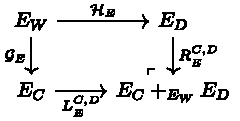
\includegraphics[width=0.95\linewidth,height=0.4\textheight,keepaspectratio]{graphic-08.pdf}\end{center}\par
 
% END S5.I1.i2.p1
 
 
\par\noindent  $\blacksquare$ 
% BEGIN S5.I1.i3.p1
 
devices $\mathcal{D}_{C\odot D}:=\mathcal{D}_{C}+\mathcal{D}_{D}$,\par
 
% END S5.I1.i3.p1
 
 
\par\noindent  $\blacksquare$ 
% BEGIN S5.I1.i4.p1
 
device assignment $\mathsf{dev}_{C\odot D}:E_{C}+_{E_{W}}E_{D}\to\mathcal{P}(\mathcal{D}_{C\odot D})$ the unique map induced by the universal property of the pushout via the assignments $\mathsf{dev}_{C}$ and $\mathsf{dev}_{D}$,\par
 
% END S5.I1.i4.p1
 
% BEGIN S5.I1.i4.p2
 
\begin{center}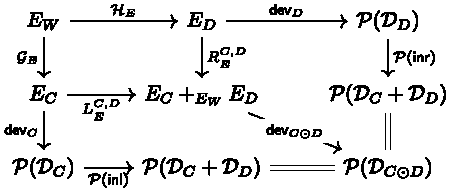
\includegraphics[width=0.95\linewidth,height=0.4\textheight,keepaspectratio]{graphic-09.pdf}\end{center}
 
% END S5.I1.i4.p2
 
 
\par\noindent  $\blacksquare$ 
% BEGIN S5.I1.i5.p1
 
$\mathcal{G\odot H}:W\to C\odot D$ is identity-on-objects and $\mathcal{G}_{E}\mathop{\fatsemi}L_{E}^{C,D}\nobreak\ (=\mathcal{H}_{E}\mathop{\fatsemi}R_{E}^{C,D})$ on arrows.\par
 
% END S5.I1.i5.p1
 
  
% END Thmtheorem43.p1
 
% END Thmtheorem43
 
% BEGIN Thmtheorem44
 
\par\medskip\noindent\textbf{Example 44.}\par
 
% BEGIN Thmtheorem44.p1
 
A simple example is given by our printer example from Section 1, reproduced in Figure 7 (left), with the chosen monoidal signature of pure actions $W$ made explicit: in this case, it comprises the only pure action, namely the “document” generator. The commuting tensor product of this effectful signature with itself is the effectful signature in Figure 7 (right), in which we have two distinct printers.\par
 
% END Thmtheorem44.p1
 
% BEGIN S5.F7

\begin{center}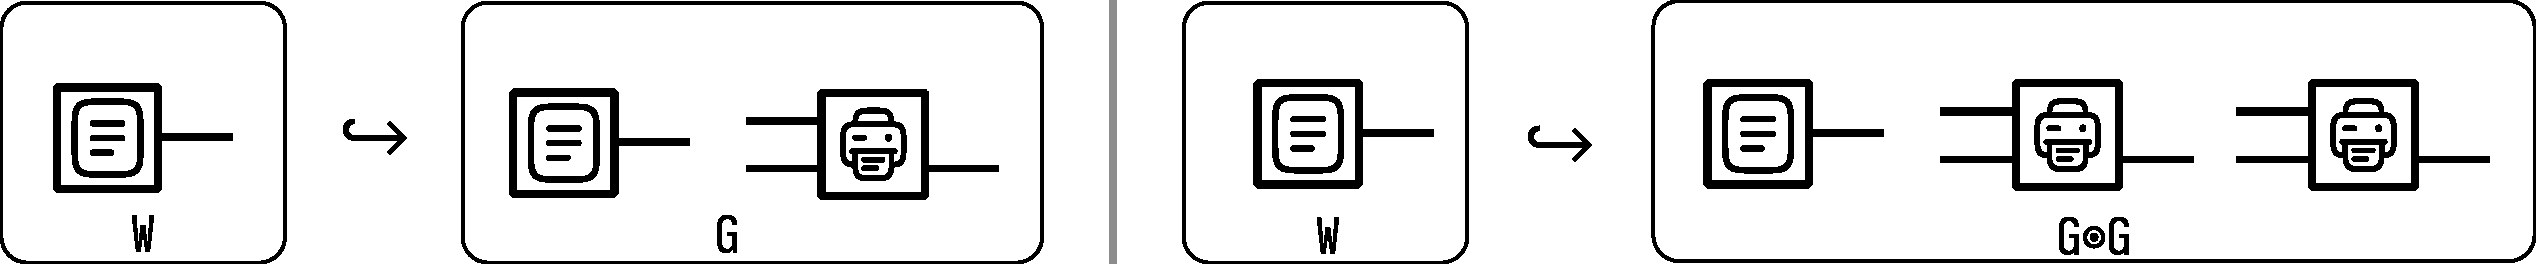
\includegraphics[width=0.95\linewidth,height=0.4\textheight,keepaspectratio]{graphic-10.pdf}\end{center}
 
Figure 7: (Left) effectful signature corresponding to the simple “theory of a printer”. (Right) Commuting tensor product of this effectful signature with itself: the theory of two printers that may be used in parallel.\par
 
% END S5.F7
 
% END Thmtheorem44
 
% BEGIN S5.p3
 
Our next goal is to show that the free effectful category over a commuting tensor product of effectful signatures is isomorphic to the commuting tensor product of the free effectful categories over those graphs. First, we recall the definition of commuting tensor product of effectful categories given by Garner and López Franco [10, §9.4], see also [6, Proposition 4.6.4]. The definition builds on the auxiliary notion of commuting cospan.\par
 
% END S5.p3
 
% BEGIN Thmtheorem45
 
\par\medskip\noindent\textbf{Definition 45 (Commuting cospan).}\par
 
% BEGIN Thmtheorem45.p1
 
A cospan of effectful categories\par
    \[F:(\mathscr{A}:\mathbb{V}\shortrightarrow\mathbb{A})\to(\mathscr{K}:\mathbb{V}\shortrightarrow\mathbb{K})\leftarrow(\mathscr{B}:\mathbb{V}\shortrightarrow\mathbb{B}):G,\]    
over the same monoidal category $\mathbb{V}$, is said to be commuting when, for every $f$ in $\mathbb{A}$ and $g$ in $\mathbb{B}$, we have $F(f)\parallel G(g)$, i.e. $F(f)$ and $G(g)$ interchange in $\mathbb{K}.$\par
 
% END Thmtheorem45.p1
 
% END Thmtheorem45
 
% BEGIN Thmtheorem46
 
\par\medskip\noindent\textbf{Definition 46.}\par
 
% BEGIN Thmtheorem46.p1
 
Let $\mathscr{A}$ and $\mathscr{B}$ be effectful categories over a monoidal category $\mathbb{V}$. The commuting tensor product of $\mathscr{A}$ and $\mathscr{B}$, denoted $\mathscr{A}\odot\mathscr{B}$, is defined to be the apex of the initial commuting cospan $L:\mathscr{A}\to\mathscr{A}\odot\mathscr{B}\leftarrow\mathscr{B}:R$ of effectful categories over $\mathbb{V}$. Explicitly, for any other commuting cospan, $F:\mathscr{A}\to\mathscr{K}\leftarrow\mathscr{B}:G$ of effectful categories over $\mathbb{V}$, there exists a unique morphism of effectful categories $\mathscr{A}\odot\mathscr{B}\to\mathscr{K}$ such that:\par
 
% END Thmtheorem46.p1
 
% BEGIN Thmtheorem46.p2
 
\begin{center}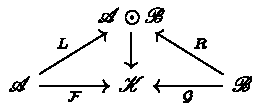
\includegraphics[width=0.95\linewidth,height=0.4\textheight,keepaspectratio]{graphic-11.pdf}\end{center}
 
% END Thmtheorem46.p2
 
% END Thmtheorem46
 

% BEGIN Thmtheorem47
 
\par\medskip\noindent\textbf{Theorem 47.}\par
 
% BEGIN Thmtheorem47.p1
 
Given effectful signatures $\mathcal{G}:W\to C$ and $\mathcal{H}:W\to D$ over the same monoidal signature $W$, $\mathscr{F}{(\mathcal{G}\odot\mathcal{H})}\cong\mathscr{F}{\mathcal{G}}\odot\mathscr{F}{\mathcal{H}}$.\par
 
% END Thmtheorem47.p1
 
% END Thmtheorem47

 
% BEGIN S5.SS0.SSS0.P0.SPx1
 
\par\medskip\noindent\textbf{Proof.}\par
 
% BEGIN S5.SS0.SSS0.P0.SPx1.p1
 
It suffices to show that $\mathscr{F}(\mathcal{G}\odot\mathcal{H})$ is the apex of the initial commuting cospan of effectful categories over the free monoidal category on $W$. In particular, we will show that:\par
 
% END S5.SS0.SSS0.P0.SPx1.p1
 
% BEGIN S5.SS0.SSS0.P0.SPx1.p2
 
\begin{center}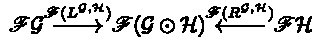
\includegraphics[width=0.95\linewidth,height=0.4\textheight,keepaspectratio]{graphic-12.pdf}\end{center}
 
% END S5.SS0.SSS0.P0.SPx1.p2
 
% BEGIN S5.SS0.SSS0.P0.SPx1.p3
 
is an initial commuting cospan, where $L^{\mathcal{G},\mathcal{H}}:\mathcal{G}\to\mathcal{G}\odot\mathcal{H}$ is the morphism of effectful signatures that is identity on objects and pure generators, and given by the left pushout injection $L^{C,D}_{E}$ on generators (Construction 43), and similarly for $R^{\mathcal{G},\mathcal{H}}:\mathcal{H}\to\mathcal{G}\odot\mathcal{H}$. This cospan is commuting because of the way in which $\mathsf{dev}_{C\odot D}$ is constructed using the universal property of the pushout given by $L^{C,D}_{E}$ and $R^{C,D}_{E}$. In particular, we have by construction that for any $x\in E_{C}$ and $y\in E_{D}$, $L^{C,D}(x)\mathrel{\bot_{C\odot D}}R^{C,D}(y)$. It follows that $\mathscr{F}(L^{\mathcal{G},\mathcal{H}})(f)\mathrel{\bot_{\mathscr{F}(\mathcal{G}\odot\mathcal{H})}}\mathscr{F}(R^{\mathcal{G},\mathcal{H}})(g)$ for any morphisms $f$ in $\mathscr{F}(\mathcal{G})$ and $g$ in $\mathscr{F}(\mathcal{H})$, from which it follows in turn that the cospan in question is commuting.\par
 
% END S5.SS0.SSS0.P0.SPx1.p3
 
% BEGIN S5.SS0.SSS0.P0.SPx1.p4
 
To see that it is initial, suppose that we have another commuting cospan of effectful categories over $\mathcal{F}_{\mathbin{\raisebox{1.25pt}{$\scriptscriptstyle\otimes$}}}W$, call it $\mathscr{F}{\mathcal{G}}\xrightarrow[]{P}(\mathscr{K}:\mathcal{F}_{\mathbin{\raisebox{1.25pt}{$\scriptscriptstyle\otimes$}}}W\shortrightarrow\mathcal{K})\xleftarrow[]{Q}\mathscr{F}{\mathcal{H}}.$ We obtain a function $(P\odot Q)_{E}:E_{C\odot D}\to E_{\mathcal{U}(\mathcal{K})}$ by the universal property of the pushout, where $\eta$ denotes inclusion of generators,\par
 
% END S5.SS0.SSS0.P0.SPx1.p4
 
% BEGIN S5.SS0.SSS0.P0.SPx1.p5
 
\begin{center}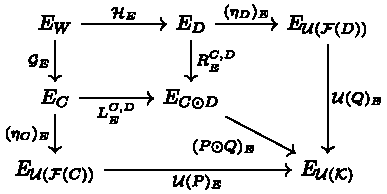
\includegraphics[width=0.95\linewidth,height=0.4\textheight,keepaspectratio]{graphic-13.pdf}\end{center}
 
% END S5.SS0.SSS0.P0.SPx1.p5
 
% BEGIN S5.SS0.SSS0.P0.SPx1.p6
 
This mapping on generators of the device signatures defines a morphism of effectful signatures $P\odot Q:\mathcal{G}\odot\mathcal{H}\to\mathscr{U}(\mathscr{K})$, where the fact that $P$ and $Q$ are a commuting cospan ensures that $f\mathrel{\bot_{\mathcal{G}\odot\mathcal{H}}}g\Rightarrow(P\odot Q)(f)\mathrel{\bot_{\mathscr{U}(\mathscr{K})}}(P\odot Q)(g)$. Using the bijection of hom-sets given by Corollary 42, we obtain a morphism $(P\odot Q)^{\#}:\mathscr{F}{(\mathcal{G}\odot\mathcal{H})}\to\mathscr{K}$ of $\mathsf{EffCat}$ such that\par
 
% END S5.SS0.SSS0.P0.SPx1.p6
 
% BEGIN S5.SS0.SSS0.P0.SPx1.p7
 
\begin{center}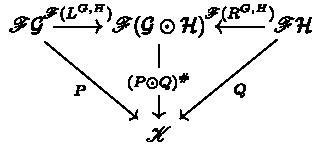
\includegraphics[width=0.95\linewidth,height=0.4\textheight,keepaspectratio]{graphic-14.pdf}\end{center}
 
% END S5.SS0.SSS0.P0.SPx1.p7
 
% BEGIN S5.SS0.SSS0.P0.SPx1.p8
 
Any other such morphism, transported back across the adjunction, induces another filler for our pushout diagram, and must therefore be equal to $(P\odot Q)^{\#}$. $\hfill\blacktriangleleft$\par
 
% END S5.SS0.SSS0.P0.SPx1.p8
 
% END S5.SS0.SSS0.P0.SPx1
 
% END S5


% BEGIN S6
 
\par\medskip\noindent\textbf{6 Conclusion and further work}\par
 
% BEGIN S6.p1
 
We have shown how morphisms in free effectful categories can be seen as generalizations of Mazurkiewicz traces, by introducing a new notion of generating data for effectful categories, namely effectful signatures. This point of view also leads to a simple presentation of the commuting tensor product of free effectful categories. In this paper, we have not given a treatment of presentations involving equations but this would be a natural next step, and would allow us to express richer descriptions of concurrent systems, such as commuting tensor products of global state [23].\par
 
% END S6.p1
 
% BEGIN S6.p2
 
Prior work has generalized Mazurkiewicz traces along different lines, such as to contextual traces [2] or semicommutations [3], so these might be investigated in light of this paper. For example, semicommutations generalize Mazurkiewicz traces by allowing commutations to be directed, and this may correspond to a notion of order-enriched effectful category.\par
 
% END S6.p2
 
% BEGIN S6.p3
 
Since effectful categories are equivalent to strong promonads [22, 10], recasting our concepts from that point of view would bring our work adjacent to the literature on combining monads [12], whose relation to the commuting tensor product should be investigated. This may also suggest appropriate generalizations. For example, we might be able to see device information as corresponding to a grading of a strong promonad.\par
 
% END S6.p3
 
% BEGIN S6.p4
 
String diagrams bearing some resemblance to resourceful traces have been used informally by Melliès in a treatment of the local state monad [18]. The local state monad arises as a combination of global state monads, linked by a theory of allocation: connections to our commuting tensor product should be investigated. Similarly, Barrett, Heijltjes, and McCusker [1] have made informal use of string diagrams bearing resemblance to resourceful traces, in which devices stand for distinct effects in an effectful $\lambda$-calculus. These instances suggest that it would be worthwhile to formalize the diagrammatic point of view. Sobociński and the third author [23] proved that string diagrams over effectful signatures with a single global device do indeed give free premonoidal categories. However, since it is possible to construct effectful categories whose interference graphs contain an infinite number of maximal cliques, making the string-diagrammatic construction formal in our setting would require restricting to an appropriate subcategory of finitary effectful signatures. With this restriction, we see no reason why string diagrams for effectful categories should not extend to our setting.\par
 
% END S6.p4
 
% END S6


% BEGIN A1
 
\par\medskip\noindent\textbf{Appendix A Omitted details}\par
 
% BEGIN A1.p1
 
% BEGIN Thmtheorem25
 
\par\medskip\noindent\textbf{Lemma 25. [Restated, see original statement.]}\par
 
% BEGIN Thmtheorem25.p1
 
Let $f,g$ be two morphisms of $\mathcal{F}G$. If $f$ and $g$ are orthogonal, $\mathsf{dev}_{\mathcal{F}G}(f)\cap\mathsf{dev}_{\mathcal{F}G}(g)=\varnothing$, then $f\parallel g$ and $g\parallel f$.\par
 
% END Thmtheorem25.p1
 
% END Thmtheorem25
 
% END A1.p1
 
% BEGIN A1.SS0.SSS0.P0.SPx1
 
\par\medskip\noindent\textbf{Proof.}\par
 
% BEGIN A1.SS0.SSS0.P0.SPx1.p1
 
By structural induction on $f$ and $g$. The cases where one of $f$ and $g$ are an identity or both morphisms are whiskered generators are straightforward by the equations of premonoidal categories, or by the imposed interchange equations for whiskered generators. Let $f=f_{1}{\mathop{\fatsemi}}f_{2}$, then by assumption we obtain $\mathsf{dev}_{\mathcal{F}G}(f_{1})\cap\mathsf{dev}_{\mathcal{F}G}(g)=\mathsf{dev}_{\mathcal{F}G}(f_{2})\cap\mathsf{dev}_{\mathcal{F}G}(g)=\varnothing$, and by hypothesis $f_{1}{\color[rgb]{0.296875,0.3359375,0.4140625}\definecolor[named]{pgfstrokecolor}{rgb}{0.296875,0.3359375,0.4140625}\parallel}g$ and $f_{2}{\color[rgb]{0.296875,0.3359375,0.4140625}\definecolor[named]{pgfstrokecolor}{rgb}{0.296875,0.3359375,0.4140625}\parallel}g$. Say $f_{1}:A\to B,f_{2}:B\to C,g:D\to E$. We need to show $((f_{1}\mathop{\fatsemi}f_{2})\rtimes D){\mathop{\fatsemi}}(C\ltimes g)=(A\ltimes g){\mathop{\fatsemi}}((f_{1}{\mathop{\fatsemi}}f_{2})\rtimes E)$. By the functoriality of $\rtimes$ and associativity of $\mathop{\fatsemi}$, the left-hand side is equal to $(f_{1}\rtimes D)\mathop{\fatsemi}((f_{2}\rtimes D)\mathop{\fatsemi}(C\ltimes g))$. Using the two induction hypotheses, this becomes $(A\ltimes g)\mathop{\fatsemi}((f_{1}\rtimes E)\mathop{\fatsemi}(f_{2}\rtimes E))$ which is finally equal to the right-hand side by the functoriality of $\rtimes$. The argument for $g||f$ is symmetric, as well as the case when $g$ is a composite. $\hfill\blacktriangleleft$\par
 
% END A1.SS0.SSS0.P0.SPx1.p1
 
% BEGIN A1.SS0.SSS0.P0.SPx1.p2
 
The following tautological construction of the free strict monoidal category on a monoidal signature is standard (see e.g. [11, Appendix A]).\par
 
% END A1.SS0.SSS0.P0.SPx1.p2
 
% BEGIN Thmtheorem48
 
\par\medskip\noindent\textbf{Construction 48 (Free strict monoidal category).}\par
 
% BEGIN Thmtheorem48.p1
 
For a monoidal signature $G$, we construct a strict monoidal category $\mathcal{F}_{\mathbin{\raisebox{1.25pt}{$\scriptscriptstyle\otimes$}}}G$ on $G$ as follows. The underlying category of $\mathcal{F}_{\mathbin{\raisebox{1.25pt}{$\scriptscriptstyle\otimes$}}}G$ has:\par
  
\par\noindent  $\blacksquare$ 
% BEGIN A1.I1.i1.p1
 
set of objects $V_{G}^{*}$, the free monoid on $V_{G}$,\par
 
% END A1.I1.i1.p1
 
 
\par\noindent  $\blacksquare$ 
% BEGIN A1.I1.i2.p1
 
set of morphisms constructed according to the following rules:\par
 
% END A1.I1.i2.p1
 
% BEGIN A1.I1.i2.p2
 
\begin{center}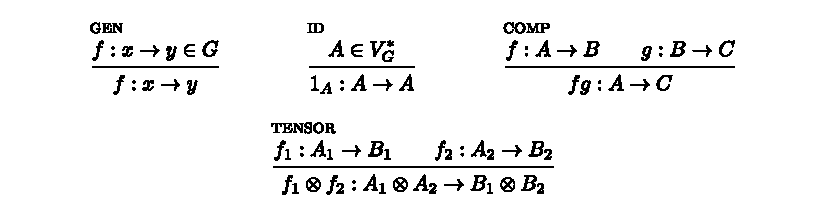
\includegraphics[width=0.95\linewidth,height=0.4\textheight,keepaspectratio]{graphic-15.pdf}\end{center}
 
subject to the equations,\par
    \[(fg)h=f(gh)\\
1_{A}f=f=f1_{B}\\
(1_{A}\otimes 1_{B})=1_{A\otimes B}\]       \[(f_{1}\otimes f_{2})(g_{1}\otimes g_{2})=(f_{1}g_{1})\otimes(f_{2}g_{2})\\
(f\otimes g)\otimes h=f\otimes(g\otimes h)\]    
% END A1.I1.i2.p2
 
 
\par\noindent  $\blacksquare$ 
% BEGIN A1.I1.i3.p1
 
composition and identities are given by the corresponding inference rules.\par
 
% END A1.I1.i3.p1
 
  
The first two equations ensure that this data forms a category and the remaining equations ensure that the evident monoidal product is functorial.\par
 
% END Thmtheorem48.p1
 
% BEGIN Thmtheorem48.p2
 
Similarly, the free strict monoidal functor on a morphism of monoidal signatures is given by the evident inductive extension.\par
 
% END Thmtheorem48.p2
 
% END Thmtheorem48
 
% BEGIN Thmtheorem49
 
\par\medskip\noindent\textbf{Proposition 49.}\par
 
% BEGIN Thmtheorem49.p1
 
The construction of $\mathcal{F}_{\mathbin{\raisebox{1.25pt}{$\scriptscriptstyle\otimes$}}}$ defines a functor $\mathcal{F}_{\mathbin{\raisebox{1.25pt}{$\scriptscriptstyle\otimes$}}}:\mathsf{MonGraph}\to\mathsf{MonCat}$.\par
 
% END Thmtheorem49.p1
 
% END Thmtheorem49
 
% BEGIN Thmtheorem50
 
\par\medskip\noindent\textbf{Definition 50.}\par
 
% BEGIN Thmtheorem50.p1
 
The underlying monoidal signature ${\color[rgb]{1,.5,0}\definecolor[named]{pgfstrokecolor}{rgb}{1,.5,0}\mathcal{U}_{\mathbin{\raisebox{1.25pt}{$\scriptscriptstyle\otimes$}}}}M$ of a monoidal category $M$ is defined to have set of objects the set of objects of $M$, and set of arrows,\par
    \[\coprod_{\begin{subarray}{c}(X_{1}\in M_{\mathsf{obj}},...,X_{n}\in M_{\mathsf{obj}})\\
(Y_{1}\in M_{\mathsf{obj}},...,Y_{m}\in M_{\mathsf{obj}})\end{subarray}}M(X_{1}\otimes...\otimes X_{n};Y_{1}\otimes...\otimes Y_{m})\]    
% END Thmtheorem50.p1
 
% BEGIN Thmtheorem50.p2
 
with the obvious assignments of sources and targets of arrows. For a strict monoidal functor $F:M\to N$, its underlying morphism of monoidal signatures $\mathcal{U}_{\mathbin{\raisebox{1.25pt}{$\scriptscriptstyle\otimes$}}}(F)$ is given by the action of $F$ on objects and arrows.\par
 
% END Thmtheorem50.p2
 
% END Thmtheorem50
 
% BEGIN Thmtheorem51
 
\par\medskip\noindent\textbf{Proposition 51.}\par
 
% BEGIN Thmtheorem51.p1
 
Definition 50 defines a functor $\mathcal{U}_{\mathbin{\raisebox{1.25pt}{$\scriptscriptstyle\otimes$}}}:\mathsf{MonCat}\to\mathsf{MonGraph}$.\par
 
% END Thmtheorem51.p1
 
% END Thmtheorem51
 
% BEGIN Thmtheorem52
 
\par\medskip\noindent\textbf{Proposition 52.}\par
 
% BEGIN Thmtheorem52.p1
 
There is an adjunction $\mathcal{F}_{\mathbin{\raisebox{1.25pt}{$\scriptscriptstyle\otimes$}}}\dashv\mathcal{U}_{\mathbin{\raisebox{1.25pt}{$\scriptscriptstyle\otimes$}}}:\mathsf{MonCat}\leftrightarrows\mathsf{MonGraph}$.\par
 
% END Thmtheorem52.p1
 
% END Thmtheorem52
 
% END A1.SS0.SSS0.P0.SPx1
 
% BEGIN A1.SS0.SSS0.P0.SPx2
 
\par\medskip\noindent\textbf{Proof.}\par
 
% BEGIN A1.SS0.SSS0.P0.SPx2.p1
 
A left adjoint to $\mathcal{U}_{\mathbin{\raisebox{1.25pt}{$\scriptscriptstyle\otimes$}}}$ is constructed via string diagrams by Joyal and Street [14]. $\hfill\blacktriangleleft$\par
 
% END A1.SS0.SSS0.P0.SPx2.p1
 
% BEGIN A1.SS0.SSS0.P0.SPx2.p2
 
% BEGIN Thmtheorem41
 
\par\medskip\noindent\textbf{Theorem 41. [Restated, see original statement.]}\par
 
% BEGIN Thmtheorem41.p1
 
The free construction of premonoidal categories over a device signature (Definition 23) is left adjoint to forming the underlying device signature of a premonoidal category (Definition 34). That is, $\mathcal{F}\dashv\mathcal{U}:\mathsf{PremonCat}\leftrightarrows\mathsf{DevGraph}.$\par
 
% END Thmtheorem41.p1
 
% END Thmtheorem41
 
% END A1.SS0.SSS0.P0.SPx2.p2
 
% END A1.SS0.SSS0.P0.SPx2
 
% BEGIN A1.SS0.SSS0.P0.SPx3
 
\par\medskip\noindent\textbf{Proof.}\par
 
% BEGIN A1.SS0.SSS0.P0.SPx3.p1
 
We begin constructing the unit, $\eta:1_{\mathsf{DevGraph}}\to\mathcal{U}\circ\mathcal{F}$. A component $\eta_{G}:G\to\mathcal{U}(\mathcal{F}(G))$ acts on objects by inclusion as a singleton list, which we again denote simply as $A$,\par
    \[(\eta_{G})_{V}:V_{G}\to V_{\mathcal{U}(\mathcal{F}(G))}:A\mapsto A.\]    
% END A1.SS0.SSS0.P0.SPx3.p1
 
% BEGIN A1.SS0.SSS0.P0.SPx3.p2
 
On arrows, recall that by definition,\par
    \[E_{\mathcal{U}(\mathcal{F}(G))}=\coprod_{\begin{subarray}{c}(X_{1}\in\mathcal{F}(G)_{\mathsf{obj}},...,X_{n}\in\mathcal{F}(G)_{\mathsf{obj}})\\
(Y_{1}\in\mathcal{F}(G)_{\mathsf{obj}},...,Y_{m}\in\mathcal{F}(G)_{\mathsf{obj}})\end{subarray}}\mathcal{F}G(X_{1}\otimes...\otimes X_{n};Y_{1}\otimes...\otimes Y_{m}),\]    
where $\otimes$ is list concatenation. Let $A_{i},B_{j}$ be elements of $V_{G}$, and $f:A_{1},...,A_{n}\to B_{1},...,B_{m}$ a morphism in $\mathcal{F}(G)$. Let us denote the coproduct injection into the component $(A_{1},...,A_{n}),(B_{1},...,B_{m})$ of $E_{\mathcal{U}(\mathcal{F}(G))}$ by $\mathsf{in}$. Then we define,\par
    \[(\eta_{G})_{E}:E_{G}\to E_{\mathcal{U}(\mathcal{F}(G))}:f\mapsto{\mathsf{in}}\triangleright f\triangleleft,\]    
where $\triangleright f\triangleleft$ denotes the primitive left-right whiskering of $f$ by the empty list, as in Definition 23. It is easy to check that this is a morphism of the underlying monoidal signatures. For the preservation of orthogonality, if $f\perp_{G}g$ then by definition $\triangleright f\triangleleft\parallel\triangleright g\triangleleft$ and $\triangleright g\triangleleft\parallel\triangleright f\triangleleft$ in $\mathcal{F}(G)$. Therefore, $\triangleright f\triangleleft$ and $\triangleright g\triangleleft$ are not connected in the interference graph of $\mathcal{F}(G)$. Now, two maps in $\mathcal{U}(\mathcal{F}(G))$ will be orthogonal as long as they do not have a device in common, but were they to share a device, they would belong to a common maximal clique and thus be connected. This is a contradiction, so they must be orthogonal, $\eta_{G}(f)\mathbin{{\color[rgb]{0.296875,0.3359375,0.4140625}\definecolor[named]{pgfstrokecolor}{rgb}{0.296875,0.3359375,0.4140625}\perp}_{\mathcal{U}(\mathcal{F}(G))}}\eta_{G}(g)$.\par
 
% END A1.SS0.SSS0.P0.SPx3.p2
 
% BEGIN A1.SS0.SSS0.P0.SPx3.p3
 
It remains to show that $\eta$ is natural. We must show that for any $\alpha:G\to H$ in $\mathsf{DevGraph}$ we have:\par
 
% END A1.SS0.SSS0.P0.SPx3.p3
 
% BEGIN A1.SS0.SSS0.P0.SPx3.p4
 
\begin{center}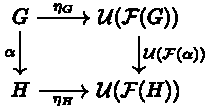
\includegraphics[width=0.95\linewidth,height=0.4\textheight,keepaspectratio]{graphic-16.pdf}\end{center}
 
% END A1.SS0.SSS0.P0.SPx3.p4
 
% BEGIN A1.SS0.SSS0.P0.SPx3.p5
 
We proceed by showing that the two above composite device signature morphisms have equal object mappings, and equal arrow mappings. First note $\mathcal{U}(\mathcal{F}(\alpha))_{V}=\alpha_{V}^{*}$ by definition, so we have,\par
    $\displaystyle((\eta_{H})_{V}\circ\alpha_{V})A=\alpha_{V}(A)=\alpha_{V}^{*}(A)$     $\displaystyle=(\alpha_{V}^{*}\circ(\eta_{G})_{V})A=(\mathcal{U}(\mathcal{F}(\alpha))_{V}\circ(\eta_{G})_{V})A$    
for all $A\in V_{G}$, as required. For the arrows, recall that by Lemma 27, $\mathcal{F}(\alpha)(\triangleright f\triangleleft)=\triangleright\alpha_{E}(f)\triangleleft$, which gives:\par
    $\displaystyle((\eta_{H})_{E}\circ\alpha_{E})f=(\eta_{H})_{E}(\alpha_{E}(f))=\mathsf{in}\nobreak\ {\triangleright}{\alpha_{E}(f)}{\triangleleft}=\mathsf{in}\nobreak\ F(\alpha)(\triangleright f\triangleleft)$     $\displaystyle=\mathcal{U}(F(\alpha))_{E}(\mathsf{in}\nobreak\ {\triangleright}{f}{\triangleleft})=\mathcal{U}(F(\alpha))_{E}(\eta_{G}f)=(\mathcal{U}(F(\alpha))_{E}\circ(\eta_{G}))f$    
establishing the naturality of $\eta:1_{\mathsf{DevGraph}}\to\mathcal{U}\circ\mathcal{F}$.\par
 
% END A1.SS0.SSS0.P0.SPx3.p5
 
% BEGIN A1.SS0.SSS0.P0.SPx3.p6
 
We now turn our attention to the counit $\varepsilon:\mathcal{F}\circ\mathcal{U}\to 1_{\mathsf{PremonCat}}$, where $\varepsilon_{\mathbb{C}}:\mathcal{F}(\mathcal{U}(\mathbb{C}))\to\mathbb{C}$ has action on objects $(\varepsilon_{\mathbb{C}})(A_{1},\ldots,A_{n}):=A_{1}\otimes\cdots\otimes A_{n}$, where $\otimes$ is the monoidal operation on objects that exists in a premonoidal category. The action on morphisms is defined by structural recursion as follows:\par
    \[\varepsilon_{\mathbb{C}}(f)=\begin{cases}1_{\varepsilon_{\mathbb{C}}(A)}&\text{ if $f=1_{A}$}\\
\varepsilon_{\mathbb{C}}(g){\mathop{\fatsemi}}\varepsilon_{\mathbb{C}}(h)&\text{ if $f=g{\mathop{\fatsemi}}h$}\\
\varepsilon_{\mathbb{C}}(X)\triangleright f^{\prime}\triangleleft\varepsilon_{\mathbb{C}}(Y)&\text{ if $f=X\triangleright\mathsf{in}f^{\prime}\triangleleft Y,$}\\
\end{cases}\]    
where $\mathsf{in}$ denotes a coproduct injection. It is straightforward to check that this is well-defined, is a monoid morphism on objects, and preserves whiskerings. It remains to show that $\varepsilon$ is natural. We must show that for any $F:\mathbb{C}\to\mathbb{D}$ in $\mathsf{PremonCat}$ we have:\par
 
% END A1.SS0.SSS0.P0.SPx3.p6
 
% BEGIN A1.SS0.SSS0.P0.SPx3.p7
 
\begin{center}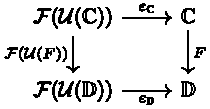
\includegraphics[width=0.95\linewidth,height=0.4\textheight,keepaspectratio]{graphic-17.pdf}\end{center}
 
% END A1.SS0.SSS0.P0.SPx3.p7
 
% BEGIN A1.SS0.SSS0.P0.SPx3.p8
 
We proceed by showing that the two composite functors have equal object mappings and equal arrow mappings. For the mapping on objects we have,\par
    $\displaystyle(F\circ\varepsilon_{\mathbb{C}})(A_{1},\ldots,A_{n})=F(A_{1}\otimes\ldots\otimes A_{n})$     $\displaystyle=F(A_{1})\otimes\ldots\otimes F(A_{n})=(\varepsilon_{\mathbb{D}}\circ\mathcal{F}(\mathcal{U}(F)))(A_{1},\ldots,A_{n}).$    
For the arrow mappings, we proceed by induction on $f$. The interesting case is when $f=X\triangleright\mathsf{in}f^{\prime}\triangleleft Y$, for $\mathsf{in}f^{\prime}$ an arrow of $\mathcal{U}(\mathbb{C})$,\par
    $\displaystyle(F\circ\varepsilon_{\mathbb{C}})(X\triangleright\mathsf{in}f^{\prime}\triangleleft Y)=F(\varepsilon_{\mathbb{C}}(X)\triangleright f^{\prime}\triangleleft\varepsilon_{\mathbb{C}}(Y))=F(\varepsilon_{\mathbb{C}}(X))\triangleright F(f^{\prime})\triangleleft F(\varepsilon_{\mathbb{C}}(Y))$     $\displaystyle=\varepsilon_{\mathbb{D}}(\mathcal{F}(\mathcal{U}(F))(X))\triangleright F(f^{\prime})\triangleleft\varepsilon_{\mathbb{D}}(\mathcal{F}(\mathcal{U}(F))(Y))$     $\displaystyle=\varepsilon_{\mathbb{D}}(\mathcal{F}(\mathcal{U}(F))(X\triangleright\mathsf{in}f^{\prime}\triangleleft Y))=(\varepsilon_{\mathbb{D}}\circ\mathcal{F}(\mathcal{U}(F)))(X\triangleright\mathsf{in}f^{\prime}\triangleleft Y).$    
The other cases follow directly from the inductive hypothesis together with the fact that each composite is a strict premonoidal functor. It follows that $\varepsilon:\mathcal{F}\circ\mathcal{U}\to 1_{\mathsf{PremonCat}}$ is natural.\par
 
% END A1.SS0.SSS0.P0.SPx3.p8
 
% BEGIN A1.SS0.SSS0.P0.SPx3.p9
 
Finally, to obtain an adjunction we must show the triangle identities:\par
    \[\begin{matrix}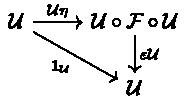
\includegraphics{graphic-18.pdf}\end{matrix}\qquad\begin{matrix}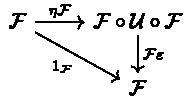
\includegraphics{graphic-19.pdf}\end{matrix}\]    
% END A1.SS0.SSS0.P0.SPx3.p9
 
% BEGIN A1.SS0.SSS0.P0.SPx3.p10
 
For the first triangle, we have:\par
    $\displaystyle(\varepsilon\mathcal{U}\circ\mathcal{U}\eta)_{\mathbb{C}}(f)=\varepsilon\mathcal{U}_{\mathbb{C}}({\eta_{\mathcal{U}\mathbb{C}}}(f))=\mathcal{U}(\varepsilon_{\mathbb{C}})(\triangleright\mathsf{in}f\triangleleft)=f=1_{\mathcal{U}(\mathbb{C})}(f),$    
from which we may conclude that the triangle in question commutes. For the second triangle, we proceed by induction on $f$. The interesting case is when $f$ is a whiskered generating arrow, $f=X\triangleright\mathsf{in}f^{\prime}\triangleleft Y$,\par
    $\displaystyle(\mathcal{F}\varepsilon\circ\eta\mathcal{F})_{G}(X\triangleright\mathsf{in}f^{\prime}\triangleleft Y)={\mathcal{F}\varepsilon_{G}}(\eta\mathcal{F}_{G}(X\triangleright\mathsf{in}f^{\prime}\triangleleft Y))$     $\displaystyle={\mathcal{F}\varepsilon_{G}}(\mathcal{F}(\eta_{G})(X\triangleright\mathsf{in}f^{\prime}\triangleleft Y))$     $\displaystyle={\mathcal{F}\varepsilon_{G}}(\mathcal{F}(\eta_{G})(X)\triangleright\mathcal{F}(\eta_{G})(\mathsf{in}f^{\prime})\triangleleft\mathcal{F}(\eta_{G})(Y)))$     $\displaystyle={\mathcal{F}\varepsilon_{G}}([X]\triangleright\eta_{G}(\mathsf{in}f^{\prime})\triangleleft[Y])$     $\displaystyle={\varepsilon_{\mathcal{F}G}}([X])\triangleright\mathsf{in}f^{\prime}\triangleleft\varepsilon_{\mathcal{F}G}([Y])$     $\displaystyle=X\triangleright\mathsf{in}f^{\prime}\triangleleft Y,$    
where for $X=X_{1},...,X_{n}$, we denote by $[X]$ the list $[X_{1}],...,[X_{n}]$. The case where $f$ is $1_{A}$ follows from the (easily checked) fact that the claim holds for the object mapping, and the case of composition follows directly from the inductive hypothesis together with the fact that the composite is a strict premonoidal functor. $\hfill\blacktriangleleft$\par
 
% END A1.SS0.SSS0.P0.SPx3.p10
 
% BEGIN A1.SS0.SSS0.P0.SPx3.p11
 
% BEGIN Thmtheorem42
 
\par\medskip\noindent\textbf{Corollary 42. [Restated, see original statement.]}\par
 
% BEGIN Thmtheorem42.p1
 
The adjunction of Theorem 41 extends to an adjunction between effectful signatures and effectful categories. That is, $\mathscr{F}\dashv\mathscr{U}:\mathsf{EffCat}\leftrightarrows\mathsf{EffGraph}.$\par
 
% END Thmtheorem42.p1
 
% END Thmtheorem42
 
% END A1.SS0.SSS0.P0.SPx3.p11
 
% END A1.SS0.SSS0.P0.SPx3
 
% BEGIN A1.SS0.SSS0.P0.SPx4
 
\par\medskip\noindent\textbf{Proof.}\par
 
% BEGIN A1.SS0.SSS0.P0.SPx4.p1
 
We shall make use of the adjunction of Theorem 41 and the adjunction between monoidal signatures and monoidal categories ([14]). Let $\mathcal{E}:V\to G$ be an effectful signature. We first define the components of the unit, namely a morphism of effectful signatures\par
    \[\eta_{\mathcal{E}}:(\mathcal{E}:V\to G)\to(\mathscr{U}\circ\mathscr{F})(\mathcal{E}:V\to G),\]    
by letting the morphism between the monoidal signatures be the unit of the adjunction between monoidal signatures and monoidal categories, $\eta^{\mathbin{\raisebox{1.25pt}{$\scriptscriptstyle\otimes$}}}_{V}:V\to\mathcal{U}_{\mathbin{\raisebox{1.25pt}{$\scriptscriptstyle\otimes$}}}\mathcal{F}_{\mathbin{\raisebox{1.25pt}{$\scriptscriptstyle\otimes$}}}V$, and the morphism between the device signatures be given by the unit $\eta_{G}:G\to\mathcal{U}\mathcal{F}G$ of the adjunction constructed in Theorem 41. It is straightforward to verify that the required square commutes.\par
 
% END A1.SS0.SSS0.P0.SPx4.p1
 
% BEGIN A1.SS0.SSS0.P0.SPx4.p2
 
Let $\mathscr{E}:\mathbb{V}\to\mathbb{C}$ be an effectful category. For the components of the counit, we define a morphism of effectful categories,\par
    \[\varepsilon_{\mathscr{E}}:(\mathscr{F}\circ\mathscr{U})\mathscr{E}\to\mathscr{E}\]    
by letting the component between the monoidal categories be given by the counit of the adjunction between monoidal signatures and monoidal categories, $\varepsilon^{\mathbin{\raisebox{1.25pt}{$\scriptscriptstyle\otimes$}}}_{\mathbb{C}}:\mathcal{F}_{\mathbin{\raisebox{1.25pt}{$\scriptscriptstyle\otimes$}}}\mathcal{U}_{\mathbin{\raisebox{1.25pt}{$\scriptscriptstyle\otimes$}}}\mathbb{C}\to\mathbb{C}$, and the morphism between premonoidal categories be given by the counit of the adjunction constructed in Theorem 41.\par
 
% END A1.SS0.SSS0.P0.SPx4.p2
 
% BEGIN A1.SS0.SSS0.P0.SPx4.p3
 
It remains to show that the unit and counit satisfy the triangle identities, which follows simply from the triangle identities of the two adjunctions involved. $\hfill\blacktriangleleft$\par
 
% END A1.SS0.SSS0.P0.SPx4.p3
 
% BEGIN A1.SS0.SSS0.P0.SPx4.p4
 
\par
 
% END A1.SS0.SSS0.P0.SPx4.p4
 
% END A1.SS0.SSS0.P0.SPx4
 
% END A1

\begin{thebibliography}{99}
\bibitem{bib-bib1} 
\par\noindent    Chris Barrett, Willem Heijltjes, and Guy McCusker.  The Functional Machine Calculus II: Semantics.  In Bartek Klin and Elaine Pimentel, editors, 31st EACSL Annual Conference on Computer Science Logic (CSL 2023), volume 252 of Leibniz International Proceedings in Informatics (LIPIcs), pages 10:1--10:18, Dagstuhl, Germany, 2023. Schloss Dagstuhl -- Leibniz-Zentrum für Informatik.  doi:10.4230/LIPIcs.CSL.2023.10.  

\bibitem{bib-bib2} 
\par\noindent    Christian Choffrut and Robert Mercas.  Contextual partial commutations.  Discrete Mathematics \& Theoretical Computer Science, 12, 2010.  

\bibitem{bib-bib3} 
\par\noindent    Mireille Clerbout and Michel Latteux.  Semi-commutations.  Information and computation, 73(1):59--74, 1987.  doi:10.1016/0890-5401(87)90040-X.  

\bibitem{bib-bib4} 
\par\noindent    Bob Coecke, Tobias Fritz, and Robert W Spekkens.  A mathematical theory of resources.  Information and Computation, 250:59--86, 2016.  doi:10.1016/J.IC.2016.02.008.  

\bibitem{bib-bib5} 
\par\noindent    Volker Diekert and Grzegorz Rozenberg.  The Book of Traces.  World Scientific, 1995.  doi:10.1142/2563.  

\bibitem{bib-bib6} 
\par\noindent    Matthew Earnshaw.  Languages of String Diagrams.  PhD thesis, Tallinn University of Technology, 2025.  doi:10.23658/TALTECH.2/2025.  

\bibitem{bib-bib7} 
\par\noindent    Matthew Earnshaw and Pawel Sobociński.  String Diagrammatic Trace Theory.  In MFCS, volume 272, 2023.  doi:10.4230/LIPIcs.MFCS.2023.43.  

\bibitem{bib-bib8} 
\par\noindent    Dominique Foata and Pierre Cartier.  Problèmes combinatoires de commutation et réarrangements.  Lecture notes in mathematics, 85, 1969.  

\bibitem{bib-bib9} 
\par\noindent    P. Freyd.  Algebra valued functors in general and tensor products in particular.  Colloquium Mathematicum, 14(1):89--106, 1966.  doi:10.4064/cm-14-1-89-106.  

\bibitem{bib-bib10} 
\par\noindent    Richard Garner and Ignacio López Franco.  Commutativity.  Journal of Pure and Applied Algebra, 220(5):1707--1751, 2016.  

\bibitem{bib-bib11} 
\par\noindent    Philip Hackney and Marcy Robertson.  On the category of props.  Applied Categorical Structures, 23(4):543--573, August 2015.  doi:10.1007/s10485-014-9369-4.  

\bibitem{bib-bib12} 
\par\noindent    Martin Hyland, Gordon Plotkin, and John Power.  Combining effects: Sum and tensor.  Theoretical computer science, 357(1-3):70--99, 2006.  doi:10.1016/J.TCS.2006.03.013.  

\bibitem{bib-bib13} 
\par\noindent    Alan Jeffrey.  Premonoidal categories and a graphical view of programs.  Preprint, 1997.  

\bibitem{bib-bib14} 
\par\noindent    André Joyal and Ross Street.  The geometry of tensor calculus, I.  Advances in Mathematics, 88(1):55--112, 1991.  doi:10.1016/0001-8708(91)90003-P.  

\bibitem{bib-bib15} 
\par\noindent    Paul Blain Levy, John Power, and Hayo Thielecke.  Modelling environments in call-by-value programming languages.  Information and Computation, 185(2):182--210, 2003.  doi:10.1016/S0890-5401(03)00088-9.  

\bibitem{bib-bib16} 
\par\noindent    Antoni Mazurkiewicz.  Concurrent program schemes and their interpretations.  DAIMI Report Series, 6(78), July 1977.  doi:10.7146/dpb.v6i78.7691.  

\bibitem{bib-bib17} 
\par\noindent    Antoni Mazurkiewicz.  Basic notions of trace theory.  In J. W. de Bakker, W. P. de Roever, and G. Rozenberg, editors, Linear Time, Branching Time and Partial Order in Logics and Models for Concurrency, pages 285--363, Berlin, Heidelberg, 2005. Springer Berlin Heidelberg.  

\bibitem{bib-bib18} 
\par\noindent    Paul-André Melliès.  Local states in string diagrams.  In Rewriting and Typed Lambda Calculi: Joint International Conference, pages 334--348. Springer, 2014.  doi:10.1007/978-3-319-08918-8\_23.  

\bibitem{bib-bib19} 
\par\noindent    John Power.  Premonoidal categories as categories with algebraic structure.  Theoretical Computer Science, 278(1):303--321, 2002.  Mathematical Foundations of Programming Semantics 1996.  doi:10.1016/S0304-3975(00)00340-6.  

\bibitem{bib-bib20} 
\par\noindent    John Power and Edmund Robinson.  Premonoidal categories and notions of computation.  Math. Struct. Comput. Sci., 7(5):453--468, 1997.  doi:10.1017/S0960129597002375.  

\bibitem{bib-bib21} 
\par\noindent    John Power and Hayo Thielecke.  Closed freyd- and $\kappa$-categories.  In Jirí Wiedermann, Peter van Emde Boas, and Mogens Nielsen, editors, Automata, Languages and Programming, pages 625--634, Berlin, Heidelberg, 1999. Springer Berlin Heidelberg.  

\bibitem{bib-bib22} 
\par\noindent    Mario Román.  Promonads and string diagrams for effectful categories.  In Applied Category Theory, volume 380 of Electronic Proceedings in Theoretical Computer Science, pages 344--361. Open Publishing Association, 2023.  doi:10.4204/EPTCS.380.20.  

\bibitem{bib-bib23} 
\par\noindent    Mario Román and Paweł Sobociński.  String diagrams for premonoidal categories.  Logical Methods in Computer Science, Volume 21, Issue 2, April 2025.  doi:10.46298/lmcs-21(2:9)2025.  

\bibitem{bib-bib24} 
\par\noindent    Sam Staton and Paul Blain Levy.  Universal properties of impure programming languages.  In Proceedings of the 40th Annual ACM SIGPLAN-SIGACT Symposium on Principles of Programming Languages, POPL ’13, pages 179--192, New York, NY, USA, 2013. Association for Computing Machinery.  doi:10.1145/2429069.2429091.  

\bibitem{bib-bib25} 
\par\noindent    Wieslaw Zielonka.  Notes on finite asynchronous automata.  RAIRO - Theoretical Informatics and Applications - Informatique Théorique et Applications, 21(2):99--135, 1987.  doi:10.1051/ITA/1987210200991.  

\end{thebibliography}
\end{document}
